% +------- CÓDIGO FONTE TCC -------+
% 	Autor: Antônio Barbosa Neto, 2017.
% 	E-mail: abneto14@gmail.com
% +--------------------------------+

% Classe do documento --> \documentclass[OPÇÕES]{CLASSE}
\documentclass[
			   a4paper, % Tipo de papel 
			   oneside, % Impressão em apenas um lado da folha
			   12pt     % Tamanho da fonte
			   ]{book}  % Classe do documento

\usepackage{dashbox}
% Pacotes --> \usepackage[OPÇÕES]{PACOTE}
\usepackage[utf8]{inputenc} % Codificação do documento (conversão automática dos acentos) 
\usepackage[brazil]{babel}  % Traduz palavras chaves para o PT-BR (ex.: abstract->resumo)
\usepackage{indentfirst}    % Indenta o primeiro parágrafo de cada seção
\usepackage{setspace}		% Possibilita a alteração do espaçamento entre linhas
\usepackage{graphicx}       % Possibilita a inserção de figuras
\usepackage{subcaption}  % Possibilita a inserção de subfiguras
\usepackage{pdfpages}       % Possibilita a inserção de páginas em pdf
\usepackage{amsmath}        % Inclui funções adicionais no ambiente matemático \eqref{•} \dfrac{•}{•}
\usepackage{amssymb} 		% Símbolos adicionais no documento \mathbb{R}
\usepackage{amsfonts}
\usepackage{amsthm}
\usepackage{mathrsfs}       % Símbolos da transformadas de Laplace e Fourier \mathscr{•}
\usepackage{float}			% Possibila posicionar tabelas e figuras em uma posição específica [H]
\usepackage[round]{natbib}% Inclui mais possibilidades de citações \citep{•}
\usepackage{fancyhdr}       % Possibilita a alteração de cabeçalho e rodapé
\usepackage{longtable}      % Possiblita a quebra de tabelas em duas páginas
\usepackage{multirow}		% Possibilita multiplas linhas em tabelas
\usepackage{array}			% Possibilita o uso do comando \newcolumntype{•}[•]
\usepackage{pdflscape}      % Possibilita a inserção de páginas em modo paisagem
\usepackage{listings}		% Possibilita inserir códigos fontes (C++, Java, ...)
\usepackage{slashbox}       % Adiciona o comando \backslashbox{•}{•} usado em tabelas
\usepackage{arydshln}       % Possibilita inserir linhas pontilhadas em tabelas 
\usepackage{adjustbox}      % Possibilita ajustar as tabelas as margens
\usepackage{rotating}       % Rotaciona tabelas
% \usepackage[alf]{abntex2cite}	% Citações padrão ABNT

\usepackage{tikz}
\usepackage{courier}
\usepackage{booktabs}     
\usepackage{svg}

\newcommand{\PR}[1]{\ensuremath{\left[#1\right]}}
\newcommand{\PC}[1]{\ensuremath{\left(#1\right)}}
\newcommand{\chav}[1]{\ensuremath{\left\{#1\right\}}}

\newcommand{\commentiury}[1]{{\color{blue}[IB: #1]}}

%\usepackage[inline]{showlabels} % Mostra os labels das equações
%\usepackage[notcite,notref]{showkeys} % Mostra todo os labels
\usepackage{lipsum} % preenchimento automático de textos

% Modifica os itens do sumário
\usepackage[nottoc,
			notlof,
			notlot]{tocbibind}

% Configura as margens das páginas
\usepackage[top    = 3cm,
			bottom = 2cm,
			left   = 3cm,
			right  = 2cm]{geometry}

% Possibilita hiperlinks no texto
\usepackage[pdftex,
			% backref,
			linktocpage = false,
			colorlinks  = true,
			linkcolor   = black,
			anchorcolor = blue,
			citecolor   = blue,
			urlcolor    = blue]{hyperref}

      
\usepackage[acronym, shortcuts]{glossaries}
\makenoidxglossaries

% Comandos auxiliares --> \nomecomando{COMANDO}{•}
\newcolumntype{C}[1]{>{\centering\let\newline\\\arraybackslash\hspace{0pt}}m{#1}} % Tabelas: {|C{2cm}|C{5cm}|}
\newcolumntype{L}[1]{>{\let\newline\\\arraybackslash\hspace{0pt}}m{#1}} % Tabelas: {|L{2cm}|L{5cm}|}
\newcommand*{\doi}[1]{DOI: \href{http://dx.doi.org/#1}{#1}} % Usado nas referencias

\setcounter{secnumdepth}{3} % Inclui a numeração de \subsubsection{•} no documento
\setcounter{tocdepth}{3}    % Inclui a \subsubsection{•} no sumário
\setstretch{1.5}			% Configura o espaçamento entre linhas \usepackage{setspace}

\pagestyle{fancy} 			% Configura a página para incluir o cabeçalho e rodapé
\lhead{{\footnotesize\leftmark}} % Cabeçalho esquerdo
\chead{}				         % Cabeçalho central
\rhead{\thepage}				 % Cabeçalho direito
\fancyfoot{}					 % Rodapé vazio

% Definição de novas cores
\definecolor{mygreen}{RGB}{0, 115, 0}
\definecolor{mylilas}{RGB}{170,55,240}
\definecolor{blue}{RGB}{41,5,195}

% \lstset{ % -> \usepackage{listings}
%   language=Matlab,
%   basicstyle=\ttfamily\small, 
%   morekeywords={matlab2tikz},
%   keywordstyle=\color{blue}, 
%   stringstyle=\color{mylilas}, 
%   commentstyle=\color{mygreen}, 
%   extendedchars=true,
%   showspaces=false,
%   showstringspaces=false,
%   numbers=left,
%   numberstyle=\tiny,
%   breaklines=true,
%   breakautoindent=true,
%   captionpos=b,
%   xrightmargin=0pt,
%   xleftmargin=15pt,
% }

\renewcommand{\lstlistingname}{Código}
\lstset{
  language=Python,
  tabsize=2,
  basicstyle=\small\linespread{1.2}\ttfamily,
  keywordstyle=\bfseries\color[gray]{0.2},
  commentstyle=\color{darkgray}\textit,
  breaklines=true,
  breakatwhitespace=false,
  extendedchars=true,
  showspaces=false,
  showstringspaces=false,
  numbers=left,
  numberstyle=\tiny,
  breaklines=true,
  breakautoindent=true,
  captionpos=b,
  xrightmargin=0pt,
  xleftmargin=15pt,
  % inputencoding=utf8,
  literate={á}{{\'a}}1 {à}{{\`a}}1 {â}{{\^a}}1 {ã}{{\~a}}1 {é}{{\'e}}1 {ê}{{\^e}}1 {ë}{{\"e}}1 {í}{{\'i}}1 {ç}{{\c{c}}}1 {Ç}{{\c{C}}}1 {õ}{{\~o}}1 {ó}{{\'o}}1 {ô}{{\^o}}1 {ú}{{\'u}}1 {δ}{{\ensuremath{\delta}}}1 {Ξ}{{\ensuremath{\Xi}}}1 {Ψ}{{\ensuremath{\Psi}}}1 {Γ}{{\ensuremath{\Gamma}}}1 {λ}{{\ensuremath{\lambda}}}1 {θ}{{\ensuremath{\theta}}}1
}

% Novos comandos --> \newcommand{COMANDO}{DEFINIÇÃO}
\newcommand{\instituicao} {
  UNIVERSIDADE FEDERAL DO AMAZONAS \\
  FACULDADE DE TECNOLOGIA \\
  ENGENHARIA DA COMPUTAÇÃO 
}
\newcommand{\titulo} {
  AVALIAÇÃO DE ESTRATÉGIAS DE ETC PARA MICRORREDES CC 
}
\newcommand{\apresentacao} {
  Monografia apresentada à Coordenação do
  Curso de Engenharia da Computação da
  Universidade Federal do Amazonas, como
  parte dos requisitos necessários à obtenção
  do título de Engenheiro de Computação.
}
\newcommand{\autor}{
  Andevaldo da Encarnação Vitório 
}
\newcommand{\local} {
  MANAUS-AM \\ 2024
}
\newcommand{\orientador} {
  Prof. Dr. Iury Valente de Bessa
}

\newtheorem{definition}{Definição}
\newtheorem{theorem}{Teorema}

% Abreviaturas e Siglas
% \renewcommand{\acrfullformat}[2]{#1~(#2)}

\newacronym{mgcc}{MGCC}{Microrrede de Distribuição em Corrente Contínua}
\newacronym[\glslongpluralkey={sistemas de distribuição de corrente contínua}]{sdcc}{SDCC}{sistemas de distribuição de corrente contínua}
\newacronym[\glslongpluralkey={recursos energéticos distribuídos}]{red}{RED}{recurso energético distribuído}
\newacronym{cc}{CC}{Corrente Contínua}
\newacronym{ca}{CA}{corrente alternada}
\newacronym{gd}{GD}{Geração Distribuída}
\newacronym[\glslongpluralkey={fontes de energia renovável}]{fer}{FER}{fonte de energia renovável}
\newacronym[\glslongpluralkey={sistemas de armazenamento de energia}]{sae}{SAE}{sistema de armazenamento de energia}
\newacronym[\glslongpluralkey={sistemas de controle em rede}]{scr}{SCR}{sistema de controle em rede}
\newacronym{mr}{MR}{Microrredes}
\newacronym{etc}{ETC}{controle acionado por eventos - do inglês, \textit{event-triggered control}}
\newacronym{etm}{ETM}{mecanismo de acionamento de eventos - do inglês, \textit{event-triggering mechanism}}
\newacronym{nmg}{NMGs}{Microrrede em Rede (do inglês, \textit{Networked Microgrid})}
\newacronym{lmi}{LMI}{Desigualdades Matriciais Lineares (do inglês, \textit{Linear Matrix Inequalities})}
\newacronym{zoh}{ZOH}{segurador de ordem zero - do inglês, \textit{zero-order mechanism}}
\newacronym[\glslongpluralkey={lineares e invariantes no tempo}]{lit}{LIT}{linear e invariante no tempo}
\newacronym[\glslongpluralkey={lineares a parâmetro variante - do inglês, \textit{lineares parameter varying}}]{lpv}{LPV}{Linear a parâmetro variante - do inglês, \textit{linear parameter varying }}
\newacronym[\glslongpluralkey={intervalos mínimos entre eventos}]{imee}{IMEE}{intervalo mínimo entre eventos}
\newacronym[\glslongpluralkey={esquemas de comunicação acionado por eventos}]{ecae}{ECAE}{esquema de comunicação acionado por eventos}
\newacronym[\glslongpluralkey={limites de tempo finito}]{ltf}{LTF}{limites de tempo finito}
\newacronym{efes}{EFES}{estabilidade finita de entrada-saída}
\newacronym{ees}{EES}{estabilidade entrada-estado}
\newacronym{cmd}{CMD}{controle por modo deslizantes}
\newacronym[\glslongpluralkey={cargas de potência constante - do inglês, \textit{constant power loads}}]{cpl}{CPL}{carga de potência constante - do inglês, \textit{constant power load}}
\newacronym{mms}{MMS}{modelo médio do sistema}
\newacronym[\glslongpluralkey={modelos de pequenos sinais}]{mps}{MPS}{modelo de pequenos sinais}
\newacronym{lkc}{LKC}{lei de Kirchoff das correntes}
\newacronym{lkt}{LKT}{lei de Kirchoff das tensões}
\newacronym{po}{PO}{ponto de operação}
\newacronym{itee}{ITEE}{intervalo de tempo entre eventos}
\newacronym{ise}{ISE}{Integral do Erro ao Quadrado - do inglês, \textit{Integral of Squared Error}}
\newacronym{itse}{ITSE}{Integral do Erro ao Quadrado Ponderado pelo Tempo - do inglês, \textit{Integral of Time-weighted Squared Error}}
\newacronym{isc}{ISC}{Integral do Controle ao Quadrado - do inglês, \textit{Integral of Squared Control}}

\newcommand{\dt}[1]{\overset{\text{\fontsize{17.28pt}{0pt}\selectfont$.$}}{#1}}

%-----------------------------------------------------
%\usepackage{ulem}
%\newcommand{\commentib}[1]{{\color{red} [IB: #1]}}
%\newcommand{\corrigir}[1]{{\color{violet}\uwave{#1}}}
%-----------------------------------------------------

\begin{document}

\begin{titlepage}
	\begin{center}
		\begin{figure}[t]
			\centering
			\includegraphics[scale=0.7]{figuras/logo_ufam.eps}
		\end{figure}

		\textbf {\instituicao}
		\vfill
		\textbf{\titulo}
		\vfill
		\textbf{\autor}
		\vfill
		\textbf{\local}

	\end{center}

\end{titlepage}

%\begin{titlepage}
	
\includepdf{parte1_pre-textuais/lombada_tcc.pdf}
		
\end{titlepage}



\thispagestyle{empty}

\begin{center}

\autor

\vfill \titulo

\vfill{
\begin{flushright}
	\begin{minipage}{8cm} 
		\apresentacao
	\end{minipage}
\end{flushright}
}

\vfill Orientador: \orientador

\vfill	\local

\end{center}

% \thispagestyle{empty}

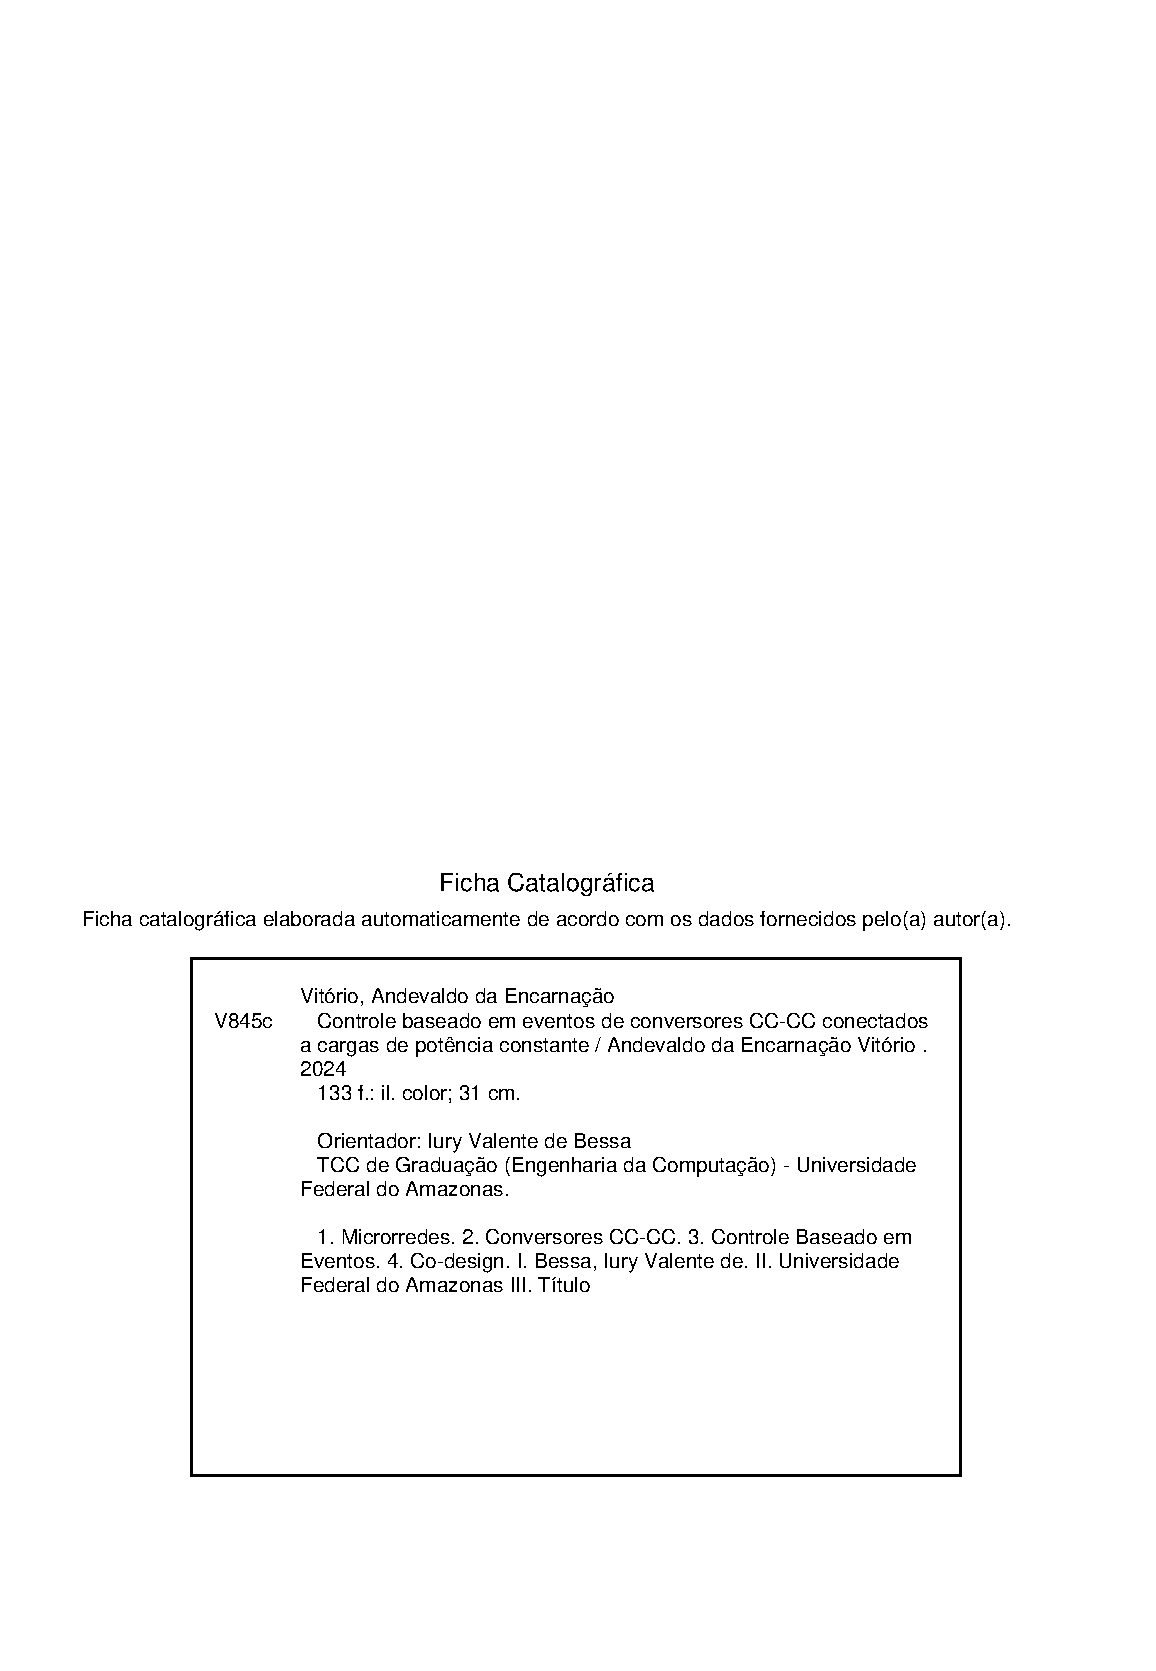
\includepdf{parte1_pre-textuais/catalografica.pdf}

% \thispagestyle{empty}

\begin{center}

\autor


\vfill	\titulo


\vfill{
\begin{flushright}
	\begin{minipage}{8cm} 
		\apresentacao
	\end{minipage}
\end{flushright}
}

\vfill	\leftline{Aprovado em 02 de abril de 2023.}


\vfill	BANCA EXAMINADORA

\vfill{
	\rule{300pt}{0.5pt} \\
	Prof. Dr. Iury Valente de Bessa -- Presidente e Orientador\\
	Departamento de Eletricidade -- UFAM
}

\vfill{
	\rule{300pt}{0.5pt} \\
	Prof. Dr. João Edgar Chaves Filho -- Membro \\
	Departamento de Eletricidade -- UFAM
}

\vfill{
	\rule{300pt}{0.5pt} \\
	Prof. Dr. Florindo Antonio Carvalho Ayres Júnior -- Membro\\
	Departamento de Eletricidade -- UFAM
}


\vfill \local

\end{center}

% \thispagestyle{empty}

\vspace*{\fill}
\begin{flushright}
	\begin{minipage}{8cm}
		\textit{
			\qquad Dedico este trabalho de conclusão de curso a todos que acreditaram em mim e me motivaram a persistir. Meu sincero agradecimento por fazerem parte dessa conquista.  
		}
	\end{minipage}
\end{flushright}

% \chapter*{Agradecimentos}
\thispagestyle{empty}

\thispagestyle{empty}

\vspace*{\fill}
\begin{flushright}
	\begin{minipage}{8cm}
		\textit{
			“O êxito da vida não se mede pelo caminho que você conquistou, mas sim pelas dificuldades que superou no caminho.”
			\\\\
			\rightline{(Abraham Lincoln)}
		}
	\end{minipage}
\end{flushright}



\chapter*{Resumo}
\thispagestyle{empty}

Adicionar resumo aqui...

\vspace{50pt}

\paragraph{Palavras-chave: ...}

\chapter*{Abstract}
\thispagestyle{empty}

Given the growing demand for sustainable and efficient energy sources, electric microgrids (MGs) with direct current (DC) assume a fundamental role in decentralizing energy generation. Characterized by distributed generation and local storage, they represent an innovative benchmark in energy management. However, the implementation of DC MGs brings challenges, especially in controlling and integrating energy resources. Additionally, electric grids have evolved, becoming increasingly smarter, and have utilized advanced technologies to optimize energy efficiency and sustainability, where communication resources play a crucial role in this process, facilitating coordination and control of network elements. However, integrating these resources can also pose challenges that need to be addressed to ensure the efficient operation of DC MGs. To ensure the proper functioning of loads and minimize losses in a DC MG, it is common to use DC-DC converters. They play a fundamental role in adapting different energy sources and loads, contributing to the autonomy and reliability of electrical systems. Faced with these challenges, a sufficient condition has been proposed for the design of event-based control strategies, using a co-design approach for Buck and Boost DC-DC converters. The application of this methodology aims to reduce the number of triggered events, ensuring stability and performance of the converters.

\vspace{50pt}



\paragraph{Keywords: Microgrids, DC-DC Converters, Event-Based Control, Co-design.} 



\pagenumbering{roman}

\listoffigures

%\thispagestyle{empty}

\listoftables

%\thispagestyle{empty}


% \markboth{\MakeUppercase{Lista de Abreviaturas e Siglas}}{\MakeUppercase{Lista de Abreviaturas e Siglas}}

% \chapter*{Lista de Abreviaturas e Siglas}

% \begin{longtable}{lL{14cm}L{\textwidth}}
  % \end{longtable}

\printnoidxglossary[type=acronym, title={Lista de Abreviaturas e Siglas}]
\printacronyms
\markboth{\MakeUppercase{Lista de Símbolos}}{\MakeUppercase{Lista de Símbolos}}

\chapter*{Lista de Símbolos}

\begin{spacing}{1.45}

\noindent \textbf{Símbolos Matemáticos}

\begin{longtable}{L{1.5cm}L{14cm}L{\textwidth}}

$\mathbb{R}$ & Conjunto dos números reais & \\



\end{longtable}

\end{spacing}

\tableofcontents




\thispagestyle{empty}


\pagenumbering{arabic}

\chapter{Introdução}

\section{Contextualização}

% Tópico: Microrredes - Introdução
Microrredes se configuram como sistemas elétricos de pequeno porte, caracterizados por geração distribuída, armazenamento e consumo local de energia. Frequentemente, integram fontes renováveis, como painéis solares e turbinas eólicas, para suprir a demanda energética local, podendo operar de maneira isolada ou conectada à rede elétrica principal. As microrredes apresentam características singularmente distintas dos sistemas de energia tradicionais, principalmente no que concerne ao controle das redes de distribuição \citep{Paigi2013}. Essa natureza peculiar impõe desafios específicos, exigindo o desenvolvimento e implementação de estratégias de controle robustas e eficazes. A seguir, exploraremos em detalhes alguns aspectos cruciais que ilustram a complexa dinâmica deste cenário dinâmico.

% Tópico: Estrutura da Microrrede
As particularidades das microrredes e os desafios de controle inerentes a elas exigem implementar um esquema hierárquico de controle. Essa estrutura, composta por três níveis distintos - primário, secundário e terciário - visa aprimorar o desempenho global da microrrede. No nível primário, o foco reside na estabilidade local. Através do monitoramento e ajuste da frequência e da tensão, os controladores primários garantem que esses parâmetros operem em limites aceitáveis \citep{Paigi2013}. O nível secundário prioriza a coordenação das unidades geradoras. Mediante mecanismos de controle, o compartilhamento eficiente de potência é estabelecido, minimizando perdas e otimizando a eficiência do sistema como um todo \cite{Paigi2013}. No nível terciário, a coordenação abrangente entre unidades geradoras e consumidores é realizada. O objetivo principal é a minimização dos custos operacionais da microrrede, buscando o equilíbrio entre geração, consumo e demanda \citep{Paigi2013}. A integração desses níveis hierárquicos demonstra um potencial significativo para aprimorar a confiabilidade, eficiência e resiliência das microrredes. Essa abordagem robusta contribui para a viabilidade e o sucesso da integração de microrredes no sistema elétrico moderno.

\textcolor{red}{[IB: Revisar todos os usos do comando \texttt{cite} e \texttt{citep}. O uso está muitas vezes incoerentes: deve-se usar o \texttt{cite} para autores e \texttt{cite} para obra!]}

% Tópico: Apresentação dos Desafios das Microrredes
Embora representem um avanço significativo na descentralização da geração de energia, as microrredes também apresentam desafios específicos no que diz respeito ao controle. A ausência de inércia rotativa, crucial nos sistemas elétricos tradicionais, é um dos principais obstáculos. Nas microrredes, a predominância de elementos interconectados eletronicamente contribui para essa falta de inércia, impactando a estabilidade do sistema \cite{Paigi2013}. Outro desafio significativo é a dependência da amplitude de tensão nas linhas de energia das redes de baixa ou média tensão. Essa característica exige estratégias de controle adaptáveis para garantir a distribuição eficiente da potência ativa \citep{Paigi2013}. Por fim, a intermitência das fontes renováveis, como a solar e a eólica, impõe um terceiro desafio. A natureza variável da geração de energia exige soluções inovadoras para o controle dinâmico da microrrede, assegurando a estabilidade e confiabilidade do sistema \citep{Paigi2013}. Superar esses desafios é fundamental para a operação eficiente das microrredes. A busca por soluções inovadoras no controle de energia elétrica torna-se crucial para o desenvolvimento e a implementação bem-sucedida dessa tecnologia.

% Tópico: Apresentação dos Desafios das Microrredes: REDs
A integração de \acrfullpl{red}, como painéis solares e turbinas eólicas, em microrredes isoladas, que operam sem conexão à rede elétrica principal, impõe desafios adicionais ao controle do sistema. A necessidade de garantir o compartilhamento eficiente de potência e a estabilidade da rede se torna ainda mais crítica nesse contexto. Esquemas de controle hierárquico com foco na provisão de reserva surgem como soluções promissoras para microrredes isoladas. A reserva, definida como a capacidade de fornecer potência adicional para compensar eventos inesperados, é crucial para a robustez do sistema.  \cite{Paigi2013}. Ela pode ser dividida em reserva pré-primária e reserva primária, ambas explorando as características dos elementos da microrrede. A reserva pré-primária, utilizando a inércia rotacional dos geradores, contribui para a estabilidade inicial da rede. Já a reserva primária envolve fontes controláveis que se ajustam em tempo real para fornecer potência adicional conforme necessário. A provisão adequada de reserva garante a continuidade do fornecimento de energia, mesmo diante de falhas ou variações na demanda, promovendo a confiabilidade e a resiliência das microrredes isoladas. \cite{Paigi2013}.

% Tópico: Redes Elétricas Inteligentes e Integração de Recursos de Comunicação
As redes elétricas inteligentes, conhecidas como \textit{smart grids}, são redes que cada vez mais são constituídas por \acrshortpl{red}, pois contribuem para a otimização da eficiência e sustentabilidade energética. \textcolor{red}{[IB: O que são as redes elétricas inteligentes? Pq são inteligentes? Acho que faltou o ponto chave que justifica o trabalho: smart grids usam intensivamente recursos modernos de telecomunicações, e por isso, o controle dessa rede se torna um problema de controle em rede.]}  No entanto, isto também apresenta desafios de controle e operação, como a restauração de frequência e tensão, o compartilhamento de potência ativa e reativa, o balanceamento do estado de carga das baterias, a operação econômica ideal e a comutação suave \cite{Zhou2020}. As microrredes surgem como soluções promissoras para superar esses desafios, possibilitando a interconexão e formação de microrredes em rede (\acrshort{nmg}, do inglês \textit{Networked Microgrids}). As \acrshort{nmg} ampliam ainda mais os benefícios das microrredes, mas exigem alta confiabilidade nas redes de comunicação entre suas unidades. Problemas de comunicação podem comprometer o desempenho do controle do sistema, resultando em perda de eficiência e instabilidade operacional. \cite{Zhou2020}.

% Tópico: Conversores CC - Introdução
Para garantir o funcionamento eficiente e estável das microrredes, a importância dos conversores \acrshort{cc}-\acrshort{cc} assume um papel crucial. Esses dispositivos desempenham a função de adaptar as características das diferentes fontes de energia e cargas conectadas à microrrede, e podem garantir a compatibilidade entre os diversos elementos da microrrede possibilitando sua integração e operação eficiente. Além de proporcionar flexibilidade operacional, os conversores \acrshort{cc}-\acrshort{cc} também contribuem para aumentar a autonomia e confiabilidade das microrredes. Isso se torna especialmente relevante em situações de operação isolada da rede elétrica principal, onde a microrrede precisa operar de forma autônoma e garantir o fornecimento de energia de forma segura e confiável. \cite{bessa2022}.

% Tópico: Conversores CC - Definição
Um sistema conversor \acrshort{cc}-\acrshort{cc} consiste em um circuito capaz de transferir energia elétrica de uma fonte de entrada para uma fonte de saída. Este circuito é composto por semicondutores de potência, que atuam como interruptores, e por elementos passivos, como indutores e capacitores, que controlam o fluxo de energia. A variável de controle fundamental do sistema é a razão cíclica, também conhecida como ciclo de trabalho. O objetivo principal do conversor \acrshort{cc}-\acrshort{cc} é regular a transferência de energia da fonte de entrada para a fonte de saída, adaptando-a às suas necessidades específicas. As fontes de entrada e saída podem variar consideravelmente, dependendo da aplicação do conversor. A carga conectada ao conversor também apresenta grande diversidade. Em alguns casos, pode ser composta por resistores. Em outros, pode ser um motor de corrente contínua, um banco de baterias, um dispositivo de soldagem elétrica a arco ou outro tipo de conversor estático. \cite{martins2008}.


% Tópico: Conversores CC - Classificação
A diversidade de topologias de conversores \acrshort{cc}-\acrshort{cc} se traduz em diversas opções para diferentes aplicações. Entre os tipos mais populares e amplamente utilizados, destacam-se: Buck, Boost, Buck-Boost, Cuk, Sepic e Zeta. Cada um possui características e funcionalidades específicas, atendendo a necessidades distintas de conversão de energia. O conversor Buck se destaca por sua simplicidade e eficiência na redução de tensão. A tensão na carga é sempre menor que a tensão da fonte de entrada. Por outro lado, o conversor Boost oferece a funcionalidade inversa, amplificando a tensão de entrada e fornecendo uma tensão mais alta na carga. Para aplicações que exigem flexibilidade na conversão de tensão, os conversores Buck-Boost, Cuk, Sepic e Zeta são soluções versáteis. Eles podem operar tanto como redutores quanto ampliadores de tensão, adaptando-se às necessidades específicas do sistema. O conversor Buck é o único que apresenta uma relação linear entre a tensão de entrada e a tensão de saída, facilitando o controle e a previsibilidade do sistema. \cite{martins2008}.

% Tópico: Controle Acionado por Evento - Introdução
Nos cenários abordados até o momento, especialmente em ambientes onde recursos de comunicação e energia são críticos, a gestão cuidadosa desses recursos se faz necessária para mitigar potenciais problemas que possam comprometer o funcionamento do sistema. Nesse contexto, o \acrfull{etc} - emerge como uma solução promissora para o gerenciamento das \acrshortpl{mr} \acrshort{cc}. Ao contrário das metodologias tradicionais que empregam intervalos de amostragem e comunicação fixos,  \textcolor{red}{ o \acrshort{etc} adapta esses processos em resposta a eventos específicos [IB: A última frase está confusa. Pq adaptar? Quais processos? Por favor, revise.]}, como mudanças na demanda de energia ou no estado da rede. Essa adaptabilidade possibilita uma utilização mais eficiente dos recursos disponíveis, reduzindo desperdícios ao realizar amostragens e comunicações somente quando necessário. Assim, o \acrshort{etc} pode contribuir significativamente para a redução do consumo de energia, da carga de comunicação e do processamento computacional dos sistemas. \cite{coutinho2021}.

% Tópico: Controle Acionado por Evento - Classificações - Dinâmico e Estático
As estratégias de \acrshort{etc} podem ser classificadas em dois tipos principais: estáticas e dinâmicas (ou adaptativas). Essa classificação se baseia na função de ativação avaliada pelo \acrshort{etm}, responsável por determinar quando os eventos de controle do sistema serão acionados. No \acrshort{etc} estático, a função de ativação é fixa e depende apenas do estado atual do sistema e do último estado transmitido. Isso significa que os eventos de controle são predefinidos e não se adaptam às mudanças nas condições do sistema. \cite{coutinho2021}. Por outro lado, no \acrshort{etc} dinâmico ou adaptativo, a função de ativação incorpora uma variável dinâmica interna adicional. Essa variável pode ser um relógio interno ou outra variável dinâmica que funciona como um relógio, e sua taxa de crescimento está relacionada ao estado do sistema. \cite{Girard2015}.

% Tópico: Controle Acionado por Evento - Classificações - Emulação e Co-design
Para o projeto de sistemas \acrshort{etc}, há duas abordagens principais distintas: emulação e co-design. A emulação divide o projeto em duas etapas: primeiro, o controlador é projetado para garantir a estabilidade e o desempenho do sistema em malha fechada, ignorando o \acrshort{etm} e a rede de comunicação. Em seguida, o \acrshort{etm} é projetado considerando o controlador pré-existente e os efeitos da rede de comunicação. Essa abordagem oferece flexibilidade no projeto do \acrshort{etm}, mas pode limitar o desempenho em malha fechada e exigir mais transmissões do que o necessário. Por outro lado, o co-design envolve o projeto simultâneo do \acrshort{etm} e da lei de controle. Essa abordagem supera as limitações da emulação e otimiza o desempenho global do sistema. No entanto, o co-design é um desafio devido a problemas de otimização não convexas ou multiobjetivo, e a análise é geralmente limitada a classes específicas de controladores e \acrshortpl{etm}. \cite{coutinho2021}.


\section{Objetivos}

\subsection{Objetivos Gerais}

Este estudo, com base nos contextos delineados acerca das \acrshortpl{mr} e dos conversores \acrshort{cc}-\acrshort{cc}, propõe avaliar diversas estratégias de \acrshort{etc} para o controle de conversores Buck e Boost. Esta proposta abrange a implementação de modelos abrangentes \textcolor{red}{[IB: Como assim "modelos abrangentes"?]} que consideram a regulação de tensão e aprimoram a qualidade de energia, visando garantir a estabilidade local, facilitar o compartilhamento eficiente de potência e otimizar a eficiência econômica, no contexto das \acrshortpl{mr}. \textcolor{red}{[IB: As últimas frases que definem o escopo do trabalho estão confusas.]} Tais contribuições exploram novas perspectivas no campo do controle e destacam a importância de estratégias formais para garantir a segurança, eficiência e adaptabilidade desses sistemas, os quais estão em constante evolução.

\subsection{Objetivos Específicos}
Para alcançar o objetivo geral, serão delineados os seguintes objetivos específicos que direcionarão as atividades do projeto:

\textcolor{red}{[IB: Acrescentar ponto e vírgula entre os itens e revisar: o que quer dizer desenvolver modelos específicos? O simulador é "do conversor" ou "dois conversores" mencionados antes? Quais tipos de ETMs? Qual forma de projeto (emulação ou co-design)? Avaliar em termos de quê? Valeria a pena acrescentar objetivo relacionado ao efeito da CPL e de incertezas na tensão de entrada?]}

\begin{enumerate}
  \item[(1)] Desenvolver modelos específicos dos conversores Buck e Boost
  \item[(2)] Implementar um simulador do conversor a partir do modelos desenvolvidos
  \item[(3)] Projetar diferentes ETMs e controladores para os conversores
  \item[(4)] Avaliar as diferentes estratégias de ETC para o controle dos conversores
\end{enumerate}

\section{Organização do Trabalho}

O restante do trabalho encontra-se estruturado em quatro capítulos descritos a seguir.

\textcolor{red}{[IB: vejo vários termos com iniciais maiúsculas abaixo. Isso é necessário? Qual o critério?]}

\begin{itemize}
    \item O Capítulo \ref{cap2}, "Revisão Bibliográfica", abrange a fundamentação teórica, destacando o Sistema de Controle ETC, Microrredes CC e LMIs. A segunda parte revisita Trabalhos Relacionados, focando em Controle Acionado por Eventos e Controle em Rede, estabelecendo bases para o projeto.
    \item O Capítulo \ref{cap3}, "Modelos e Protótipo", destaca a criação de modelos específicos para microrredes CC e aborda o desenvolvimento do protótipo, essencial para a implementação e teste das estratégias de Controle Acionado por Eventos propostas.
    \item O Capítulo \ref{cap4}, "Avaliação de ETC", concentra-se na análise e avaliação das estratégias de Controle Acionado por Eventos (ETC) implementadas. Este capítulo examina o desempenho das estratégias em microrredes de corrente contínua, considerando métricas como eficiência energética, confiabilidade do sistema e adaptabilidade às condições operacionais.
    \item  O Capítulo \ref{cap5}, "Conclusão", apresenta as principais descobertas do projeto, destacando conclusões derivadas da avaliação das estratégias de Controle Acionado por Eventos em microrredes de corrente contínua.
\end{itemize}



% Fim Capítulo
\chapter{Revisão Bibliográfica} \label{cap2}

\section{Fundamentação Teórica}

\subsection{Estabilidade no sentido \textit{Lyapunov}}

% Introdução do teorema de Lyapunov
Os métodos de análise de estabilidade desenvolvidos por \textit{Lyapunov} são geralmente reconhecidos como base para a compreensão da estabilidade em sistemas dinâmicos. No ano de 1892, o matemático e engenheiro russo, \textit{Aleksandr Mikhailovich Lyapunov} (1857-1917), propôs abordagens que desempenham um papel crucial na compreensão e caracterização da estabilidade dos sistemas no ponto de equilíbrio. \cite{lyapunov1892}. Em essência, ela se concentra na análise do comportamento das soluções de sistemas dinâmicos em torno de pontos de equilíbrio, estabelecendo critérios para determinar a estabilidade desses pontos, sejam eles estáveis, instáveis ou assintoticamente estáveis. Desta forma, oferece métodos sistemáticos para avaliar a estabilidade de sistemas, tanto autônomos quanto não autônomos, abrangendo desde sistemas lineares até não lineares. \cite{khalil2002}. Ao fornecer condições suficientes para a estabilidade, os métodos de \textit{Lyapunov} oferecem uma estrutura poderosa para analisar e projetar sistemas dinâmicos com garantias de estabilidade desejadas.

% Bases para o teorema de Lyapunov
Considere o sistema dinâmico representado por \begin{equation}\dot{x} = f(x), \end{equation} onde $f: D \rightarrow \mathbb{R}^n$ é um mapeamento local \textit{Lipschitz} do domínio $D \subset \mathbb{R}^n$ em $\mathbb{R}^n$, e assuma que $\bar{x} \in D$ seja o ponto de equilíbrio do sistema, ou seja, $f(\bar{x}) = 0$. Dada a capacidade de transladar qualquer ponto de equilíbrio para a origem através de mudanças de variáveis, podemos, sem perda de generalização, definir a estabilidade do sistema em relação ao ponto de equilíbrio na origem, ou seja, $\bar{x} = 0$. Assim, podemos apresentar a definição da estabilidade do ponto de equilíbrio, conforme Khalil. \cite{khalil2002}.

\begin{definition}
  O ponto de equilíbrio $\bar{x} = 0$ é

  \begin{enumerate}
    \item[$\bullet$] estável se, para cada $\epsilon > 0$, existe $\delta = \delta(\epsilon) > 0$, tal que,
          $$ \lVert x(0)\rVert < \delta \Rightarrow \lVert x(t)\rVert < \epsilon, \hspace{0.3cm} \forall \, t \geq 0$$
    \item[$\bullet$] instável, se não for estável.
    \item[$\bullet$] assintoticamente estável, se for estável e $\delta$ possa   ser escolhido de forma que:
          $$ \lVert x(0)\rVert < \delta \Rightarrow \lim_{t \rightarrow \infty}x(t) = 0$$
  \end{enumerate}
\end{definition}

Portanto, para demostrar que o ponto de equilíbrio $\bar{x} = 0$ é estável, para qualquer valor de $\epsilon$, deve-se obter um valor de $\delta$, possivelmente dependente de $\epsilon$, de modo que uma trajetória que comece em uma vizinhança $\delta$ da origem nunca sairá da vizinhança $\epsilon$. \cite{khalil2002}.

Khalil, em seu livro \textit{Nonlinear Systems}, demonstrou que a estabilidade do ponto de equilíbrio de um sistema de pêndulo pode ser compreendida através do uso de conceitos de energia. Ele definiu a energia do pêndulo como a soma de suas energias potencial e cinética, com a escolha da referência da energia potencial de modo que a energia do pêndulo na origem seja nula. Ao desconsiderar o atrito, tornando o sistema conservativo e, consequentemente, mantendo a energia do sistema constante, observou-se a formação de um contorno fechado em torno do ponto de origem, especialmente para pequenos valores de energia do sistema. Assim, o ponto de origem é identificado como um ponto de equilíbrio estável. Para sistemas dissipativos, nos quais a energia do sistema diminui ao longo do tempo, ele observou que o sistema converge para a origem conforme o tempo tende ao infinito. Portanto, é possível determinar a estabilidade do ponto de equilíbrio analisando a derivada da função energia ao longo das trajetórias do sistema. \cite{khalil2002}.

Em 1892, Lyapunov afirmou que outras funções, além da energia, podem ser utilizadas para determinar a estabilidade do ponto de equilíbrio. \cite{lyapunov1892}. Dado $V : D \rightarrow \mathbb{R}$ uma função contínua diferenciável definida no domínio $D \subset \mathbb{R}^n$ que contém o ponto de origem. A derivada da função $V$ ao longo da trajetória de $f(x)$, denotado por $\dot{V}(x)$, demostrada por Khalil, \cite{khalil2002}, é dada por:

$$ \dot{V}(x) = \frac{\partial V}{\partial x}f(x) $$

Se $\phi(t;x)$ é a solução de $f(x)$ que inicia no estado inicial $x$ no tempo $t = 0$, então:

$$ \dot{V}(x) = \left. \frac{d}{dt}f(\phi(t;x))\right|_{t=0} $$

Portanto, se $\dot{V}(x)$ é negativo, $V$ decresce ao longo da solução de $f(x)$.

% Esta é um boa forma de apresentar o teorema?
Com base nos conceitos apresentados até o momento, o teorema de estabilidade de Lyapunov pode ser definido como:

\begin{theorem}
  Seja $x = 0$ o ponto de equilíbrio para f(x) e seja $D \subset \mathbb{R}^n$ um domínio contendo $x = 0$. Seja $V : D \rightarrow \mathbb{R}$ uma função diferenciável contínua tal que:
  \begin{gather}
    V(0) = 0 \quad \text{e} \quad V(x) > 0 \quad \mathrm{em} \quad D - \{0\} \label{eq:lyapunov1} \\
    \dot{V}(x) \leq 0 \quad \mathrm{em} \quad D - \{0\} \label{eq:lyapunov2}
  \end{gather}
  Então, $x=0$ é estável. Além disto, se
  \begin{equation}
    \dot{V}(x) < 0 \quad \mathrm{em} \quad D - \{0\} \label{eq:lyapunov3}
  \end{equation}
  então, $x=0$ é assintoticamente estável.
\end{theorem}

%  Definição das função de Lyapunov, superfície de Lyapunov, e função DP e SDP.
Uma função $V(x)$ é chamada de função de Lyapunov quando é contínua e diferenciável, satisfazendo as equações \eqref{eq:lyapunov1} e \eqref{eq:lyapunov2}. A superfície $V(x) = c$, para qualquer $c > 0$, é referida como superfície de Lyapunov. Se $V(x)$ atende à condição \eqref{eq:lyapunov2}, isto é, $V(0) = 0$ e $V(x) > 0$ para $x \neq 0$, ela é considerada definida positiva. No caso em que $V(x)$ satisfaz $V(x) \geq 0$ para $x \neq 0$, ela é denominada semidefinida positiva. Uma função $V(x)$ é classificada como definida negativa ou semidefinida negativa se $-V(a)$ é definida positiva ou semidefinida positiva, respectivamente. Se $V(x)$ não se enquadra em nenhum desses casos, é considerada indefinida. Com essa terminologia, o teorema de Lyapunov pode ser reformulado, indicando que a origem é estável se existe uma função $V(x)$ definida positiva, continuamente diferenciável, tal que $\dot{V}(x)$ seja semidefinida negativa. Além disso, a estabilidade assintótica é alcançada quando $\dot{V}(x)$ é definida negativa. \cite{khalil2002}.

%  Definição das Matrizes SDP E DP
Uma classe de funções escalares para as quais a determinação do sinal pode ser facilmente realizada é a classe das funções quadráticas, representadas por:

\begin{equation}
  V(x) = x^T P x = \sum_{i=1}^n \sum_{j=1}^n p_{ij} x_i x_j
  \label{eq:lyapunov4}
\end{equation}

\noindent onde $P$ é uma matriz real simétrica. Nesse caso, $V(x)$ é positiva definida ou positiva semidefinida se, e somente se, todos os autovalores de $P$ são positivos ou não negativos, o que ocorre se e somente se todos os menores principais de $P$ são positivos ou não negativos, respectivamente. Se $V(x) = x^T P x$ é positiva definida ou positiva semidefinida, dizemos que a matriz $P$ é positiva definida ou positiva semidefinida, representado por $P > 0$ ou $P \geq 0$, respectivamente. \cite{khalil2002}.

%  To-do: adicionar um conclusão e uma ponte para LMIs
\subsection{Desigualdades Matriciais Lineares}

% Introdução às LMIs
As desigualdades matriciais lineares (\acrshortpl{lmi}, do inglês \textit{Linear Matrix Inequalities}) são de grande importância na teoria de controle e sistemas, fornecendo uma estrutura significativa para a formulação e resolução de uma variedade de problemas. Este conjunto de técnicas permite a representação de restrições complexas em termos de desigualdades lineares entre matrizes, possibilitando a abordagem de questões como estabilidade, desempenho e síntese de controladores de forma unificada. \cite{boyd1994}.

Os métodos de Lyapunov tradicionalmente empregados na análise de estabilidade de sistemas dinâmicos têm sido estendidos para permitir a formulação de \acrshortpl{lmi}, proporcionando assim uma base teórica sólida para a resolução de problemas de otimização e controle. Essa conexão entre \acrshortpl{lmi} e Lyapunov não apenas simplifica a análise e a síntese de sistemas complexos, mas também oferece uma estrutura matemática para abordar uma variedade de questões de controle de forma eficiente e sistemática. \cite{boyd1994}.

% História das LMIs
Como discutido na seção anterior, Lyapunov introduziu seus teoremas, estabelecendo que um sistema dinâmico \begin{equation} \dot{x}(t) = Ax(t) \label{eq:sys1}\end{equation} é assintoticamente estável se, e somente se, as condições descritas nas equações \eqref{eq:lyapunov1} e \eqref{eq:lyapunov3} forem satisfeitas. Adicionalmente, ele propôs uma classe de funções de Lyapunov que atendem a essas condições, conforme apresentado na equação \eqref{eq:lyapunov4}. Substituindo esta equação nas condições de estabilidade, obtemos: \begin{equation} \dot{V}(x) = \dot{x}^TPx + x^TP\dot{x} \label{eq:lyapunov5}. \end{equation} A partir do sistema (\ref{eq:sys1}), a equação (\ref{eq:lyapunov5}) pode ser reescrita como: \begin{equation} \dot{V}(x) = x^TA^TPx + x^TPAx \label{eq:lyapunov6}. \end{equation} logo, \begin{equation} \dot{V}(x) = x^T (A^TP + PA) x \label{eq:lyapunov6}, \end{equation} ou seja, o sistema (\ref{eq:sys1}) é assintoticamente estável se, e somente se, existir uma matriz definida positiva $P$ tal que \begin{equation} A^T P + P A < 0.\end{equation}

Essa condição, conhecida como desigualdade de Lyapunov em $P$, é uma forma específica de \acrshort{lmi}. Lyapunov também demonstrou que essa LMI inicial poderia ser resolvida explicitamente. Na prática, é possível escolher qualquer $Q = Q^T > 0$ e resolver a equação linear $A^T P + P A = -Q$ para a matriz $P$. Se o sistema for estável, a matriz $P$ resultante será definida positiva. Assim, a desigualdade de Lyapunov foi a primeira \acrshort{lmi} utilizada para analisar a estabilidade de sistemas dinâmicos, oferecendo uma solução analítica por meio da resolução de um conjunto de equações lineares. \cite{lyapunov1892,boyd1994}.

Após os trabalhos iniciais de Lyapunov, na década de 1940, pesquisadores soviéticos como Lur'e e Postnikov aplicaram seus métodos em problemas práticos de controle, focando especialmente na estabilidade de sistemas com não-linearidades nos atuadores. Embora suas soluções fossem resolvidas manualmente e aplicáveis apenas a sistemas menores, esse trabalho foi crucial para demonstrar a viabilidade das ideias de Lyapunov na engenharia de controle. O avanço seguinte, nos anos 1960, trouxe métodos gráficos mais acessíveis, expandindo o alcance para sistemas mais complexos e estabelecendo as bases para a resolução computacional das LMIs, marcando assim uma nova fase na teoria do controle. \cite{boyd1994}.

% Definição de um LMI
A seguir, é apresentado o conceito formal de uma \acrshort{lmi}, conforme definido por Boyd et al. \cite{boyd1994}.

\begin{definition}
  Uma \acrshort{lmi} é expressa pela equação \begin{equation} F(x) \triangleq F_0 + \sum_{i=0}^{m}(x_iF_i) > 0 \label{eq:lmi1}\end{equation} onde $x \in \mathbb{R}^m$ é a variável e as matrizes simétricas $F_i \in \mathbb{R}^{n \times n}, \, i = 0, . . . , m$, são fornecidas. Nesta expressão, o símbolo de desigualdade indica que $F(x)$ é definida positiva. Além disso, há \acrshortpl{lmi} não estritas, representadas pela forma \begin{equation} F(x) \geq 0 \end{equation}
\end{definition}

Múltiplas \acrshortpl{lmi}  $F_{(1)}(x) > 0, \, ..., \, F_{(p)}(x) > 0$ podem ser expressas como uma única \acrshort{lmi} $\mathbf{diag}(F_{(1)}(x), \, ..., \, F_{(p)}(x)) > 0$. Além disto, quando as matrizes $F_i$ são diagonais, a LMI $F(x) > 0$ é apenas um conjunto de desigualdades lineares. As desigualdades não lineares (convexas) são convertidas para a forma LMI usando complementos de Schur.

A \acrshort{lmi} \eqref{eq:lmi1} é uma restrição convexa em $x$, tornando o conjunto $\{x \, : \, F(x) > 0\}$ convexo e pode representar uma ampla variedade de restrições convexas em $x$, incluindo desigualdades lineares, quadráticas, de norma de matriz, bem como restrições comuns em teoria de controle, como desigualdades matriciais quadráticas convexas e de Lyapunov. \cite{boyd1994}.

\subsection{Sistemas de Controle Baseado em Eventos}

% ETC: Introdução
O \acrfull{etc}, surgindo como uma solução, se destaca em \acrfullpl{scr}, onde conectam componentes como sensores, controladores e atuadores através de uma rede compartilhada. Enquanto os \acrshortpl{scr} geralmente adotam o controle periódico, o que pode causar congestionamentos e desperdícios de recursos, o \acrshort{etc} executa tarefas apenas quando necessárias, minimizando estes problemas. Ele pode ser modelado de diversas formas, com destaque para o modelo de atraso de tempo, que permite lidar com atrasos de transmissão e otimizar ganhos de controle. Esses modelos despertam interesse entre pesquisadores, especialmente em estudos de estabilidade e design de controladores \cite{peng2018}.

O modelo de um sistema dinâmico em loop fechado com um \acrshort{etc} implementado pode ser descrito como um modelo típico de controle de feedback de estado, conforme ilustrado na figura a seguir.

\begin{figure}[H]
  \centering
  % \vspace{3ex}
  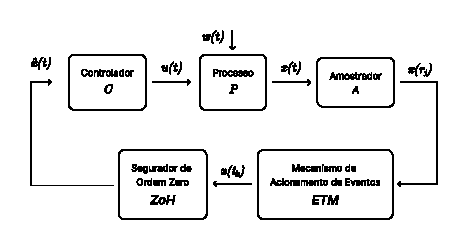
\includegraphics[scale=2.]{figuras/etc-model.eps}
  \caption{Modelo de um sistema dinâmico em loop fechado com ETC.}
  \label{fig:etc-model}
\end{figure}

% ETC: Estrutura
O modelo apresentado na \autoref{fig:etc-model} consiste em uma planta $ P$ que recebe uma entrada de perturbação não controlada $w(t)$ e a entrada de controle $u(t)$, e cujo estado é determinado por uma equação diferencial \begin{equation}\dot{x}(t) = f(x(t), u(t), w(t))\end{equation} A informação do estado pode ser monitorada de forma contínua ou amostrada, o que caracteriza o \acrshort{etc} como contínuo ou periódico, respectivamente. No caso do \acrshort{etc} periódico, um sistema de amostragem é introduzido para gerar uma sequência discreta de estados $x(t_A)$, onde o $t_A$ é o tempo de liberação do estado medido. Por outro lado, no \acrshort{etc} contínuo, o estado medido é enviado diretamente para o \acrshort{etm}. \cite{peng2018,coutinho2021,Lemmon2010}.

O \acrshort{etm} determina o instante apropriado para transmitir o estado para o \acrfull{zoh} - que é utilizado para transformar o sinal discreto resultante em um sinal contínuo no tempo,  para estar disponível para o controlador $C$ que irá mapear esses estados amostrados em um sinal de controle e aplicar à planta. \cite{coutinho2021}.

% ETC: Diferentes Abordagens - Introdução e Abordagem por Emulação
O projeto eficiente tanto do \acrshort{etm} quanto das leis de controle é crucial para assegurar o desempenho adequado e a estabilidade dos sistemas \acrshort{etc} em malha fechada. Como resultado, os modelos de \acrshort{etc} frequentemente adotam abordagens baseadas em emulação ou co-design para atingir tais objetivos. \cite{coutinho2021, peng2018}. As abordagens baseadas em emulação são geralmente realizadas em dois passos distintos. Primeiramente, um controlador é projetado para garantir a estabilidade ou um desempenho específico para o sistema em malha fechada, assumindo a ausência do \acrshort{etm} e da rede de comunicação. Este controle é projetado de acordo com uma estrutura convencional de dados amostrados periódicos, aproveitando os resultados proveitosos dos sistemas de dados amostrados. \cite{coutinho2021,peng2018}. Em seguida, o segundo passo envolve a consideração da presença do \acrshort{etm} e dos efeitos induzidos pela rede de comunicação, a fim de projetar o \acrshort{etm} de forma a preservar as propriedades garantidas pelo controlador previamente projetado. Esta abordagem permite que o \acrshort{etm} seja projetado separadamente do controle, conferindo flexibilidade no processo de projeto. \cite{coutinho2021,peng2018}. No entanto, essa independência pode limitar o desempenho em malha fechada do sistema \acrshort{etc} e exigir mais transmissões do que o necessário, uma vez que o \acrshort{etm} pode não estar otimizado para o controle específico. \cite{coutinho2021}.

% ETC: Diferentes Abordagens - Abordagem por Co-design
As abordagens baseados no \textit{co-design} buscam superar as limitações das abordagens baseadas em emulação, permitindo o design simultâneo do \acrshort{etm} e da lei de controle. No entanto, o \textit{co-design} enfrenta desafios como problemas de otimização não-convexos ou multiobjetivo, devido a restrições conflitantes de desempenho e aumento dos tempos entre eventos. A análise muitas vezes se limita a classes específicas de controladores e \acrshortpl{etm} \cite{coutinho2021}. Diferentes estratégias de \textit{co-design} têm sido desenvolvidas para várias formas de \acrshortpl{etm}. Estas incluem \textit{co-design} estático para estabilização local de sistemas LTI e \textit{co-design} dinâmico para sistemas lineares com entradas não lineares limitadas, entre outros. As condições de \textit{co-design} são frequentemente derivadas usando formalismos de sistema híbrido e expressas em termos de \acrshortpl{lmi}, permitindo uma eficiente resolução por métodos de otimização convexa \cite{coutinho2021}.

% ETC: ETM estático e dinâmico (adaptativa)
Os modelos de \acrshort{etm} podem ser diferenciados em termos da lei de acionamento, que pode ser estática ou adaptativa (dinâmica). No contexto do \acrshort{etm} estático, os instantes de transmissão são determinados com base em uma função de acionamento estática. Destaca-se, a título de ilustração, o \acrshort{etc} contínuo estático proposto por Tabuada \cite{Tabuada2007}, esclarecendo sua eficácia para sistemas não lineares em malha fechada, onde a estabilidade é garantida por meio de uma função \acrfull{ees} de \textit{Lyapunov}.

Para reduzir o número de eventos transmitidos, foram propostas funções de acionamento aprimoradas \cite{Wang2020,Zong2023,Ge2017, Ning2018, Wu2021}, introduzindo variáveis dinâmicas. Uma alternativa é considerar uma função de ponderação variável no tempo, caracterizando o \acrshort{etc} adaptativo ou dinâmico, desenvolvido principalmente no contexto de sistemas \acrshort{etc} periódico \cite{coutinho2021}. Este método permite ajustar dinamicamente o limite de acionamento, proporcionando uma adaptação mais flexível às condições do sistema. A estabilidade do sistema sob o \acrshort{etc} adaptativo é analisada usando uma função de \textit{Lyapunov} modificada, demonstrando sua eficácia em manter a estabilidade em malha fechada \cite{coutinho2021}.

% ETC: Conclusão
As diferentes abordagem de \acrshort{etc} abrangem investigações em controladores de retroalimentação de estado, observadores, \acrshortpl{etm} estáticos e dinâmicos, com o intuito de assegurar a estabilidade e o desempenho em malha fechada em uma variedade de sistemas, tais como sistemas \acrfullpl{lit} \cite{Zong2023,Wu2021}, sistemas de \textit{Lur'e} \cite{Zhang2017} e modelos \textit{fuzzy Takagi-Sugeno} \cite{Pan2017}. O foco está em estabelecer condições práticas e numericamente solucionáveis que simplifiquem o projeto eficaz de sistemas de controle complexos.

% ---------------------------------------------------------------------------
\section{\acrshort{etm} Dinâmico e Estático}

% ETM: Apresentação do trabalho de Coutinho
Em sua pesquisa, Coutinho investigou um modelo de \acrshort{etm} dinâmico e estático, sobre o qual este projeto se fundamenta. Este modelo baseia-se em uma condição suficiente para permitir o projeto simultâneo do \acrshort{etm} e do controlador com ganhos escalonados, por meio da abordagem por co-design, garantindo a estabilidade assintótica da origem do sistema em malha fechada. Além disso, aborda um problema de otimização visando a ampliação dos intervalos entre eventos, com o objetivo de minimizar a quantidade de eventos gerados pelo \acrshort{etm}. \cite{coutinho2021}.

% ETM: Apresentação do sistema dinâmico
O modelo proposto por Coutinho para o \acrshort{etm} dinâmico considera uma classe específica de sistemas não lineares, representada pela equação diferencial abaixo: \begin{equation} \dot{x}(t) = A(x(t))x(t) + B(x(t))u(t). \label{eq:etm-sys}\end{equation} Nesta equação, $ x(t) \in D \subset \mathbb{R}^n $ representa o estado do sistema, $ u(t) \in \mathbb{R}^m $ é a entrada de controle, e $ A: D \rightarrow \mathbb{R}^{n \times n} $ e $ B: D \rightarrow \mathbb{R}^{n \times m} $ são funções contínuas de matriz, com a restrição de que $ B(x) \neq 0 $ para todo $ x \in D $. Os termos não lineares nos coeficientes dependentes do estado, $ A(x) $ e $ B(x) $, são representados por $ z_j: D \rightarrow \mathbb{R} $, onde $ j \in \mathbb{N}_{\leq p} $, e são denominados funções de escalonamento. Aqui, $ D \subset \mathbb{R}^n $ é um politopo convexo que inclui a origem, sendo esta considerada o ponto de equilíbrio de interesse. \cite{coutinho2021}.

% Definição das funções de escalonamento e de ponderamento
% Warning Este texto é praticamente igual a do Coutinho
Dado que as funções de escalonamento $z_j(x)$ são contínuas e $D$ é um conjunto compacto, podemos inferir a existência de limites, de forma que: \begin{equation} z_{j}^0 \leq z_j(x) \leq z_{j}^0, \quad \forall j \in \mathbb{N}_{\leq p}. \end{equation} Assim, cada função de escalonamento $z_j(x)$ pode ser representada de maneira equivalente como: \begin{equation} z_j(x) = w_0^j(x)z_j^0 + w_{1}^j(x)z_{j}^1 = \sum_{i_j=0}^{1} w_{i_j}^j(x)z_i^{i_j}, \end{equation} onde as funções de ponderação dependentes do estado são definidas como: \begin{equation} w_0^j(x) := \frac{z_j^1 - z_j(x)}{z_j^1 - z_j^0}, \quad w_1^j(x) := 1 - w_0^j(x), \end{equation} com $0 \leq w_i^j(x) \leq 1$, $i_j \in \mathbb{B}$, $j \in \mathbb{N}_{\leq p}$. Portanto, para todo $x \in D$, o sistema não linear \eqref{eq:etm-sys} pode ser equivalente ao seguinte modelo quasi-LPV poliédrico: \begin{equation} \dot{x}(t) = \sum_{i \in \mathbb{B}_p} w_i(x(t))(A_i x(t) + B_i u(t)), \label{eq:etm-politopic} \end{equation} onde os parâmetros dependentes do estado são definidos como: \begin{equation} w_i(x) := \prod_{j=1}^{p} w_{ij}^j(x), \end{equation} sendo $i = (i_1, ..., i_p) \in \mathbb{B}_p$. Por definição, observamos que a propriedade de soma convexa permanece válida para os parâmetros: \begin{equation} \sum_{i \in \mathbb{B}_p} w_i(x) = 1, \quad 0 \leq w_i(x) \leq 1, \quad \forall i \in \mathbb{B}_p, \end{equation} garantindo que as matrizes: \begin{equation} \left. A_i := A(x) \right|_{w_i(x)=1}, \quad \left.B_i := B(x) \right|_{w_i(x)=1}, \end{equation} definem os vértices do modelo quasi-LPV poliédrico \eqref{eq:etm-politopic}. \cite{coutinho2021}.

% ETM: Lei de controle 
A seguinte lei de controle de realimentação de estado, com ganhos escalonados, é considerada para estabilizar o sistema \eqref{eq:etm-sys}:
\begin{equation} u(t) = K(\hat{x}(t))\hat{x}(t) = \sum_{j \in Bp} w_j(\hat{x}(t))K_j\hat{x}(t) \end{equation} onde $ \hat{x}(t) $ representa a informação de estado disponível para o controlador através do ETM. A matriz dependente de estado $ K : D \rightarrow \mathbb{R}^{m \times n} $ é assumida como dependente das funções de escalonamento de \eqref{eq:etm-sys}, de modo que um controlador programado para ganho com ganhos $ K_j = K(\hat{x}) $ possa ser parametrizado em termos dos parâmetros $ w_j(\hat{x}) $. \cite{coutinho2021}.

% ETM: Apresentação do erro de transmissão
Quando uma amostra de dados é transmitida no tempo do evento $t_k$, o estado disponível para o controlador é atualizado para $\hat{x}(t) = x(t_k)$, para todo $t \in [t_k, t_{k+1})$. Como é utilizado um \acrshort{zoh}, $\hat{x}(t)$ é mantido constante até o próximo tempo de evento $t_{k+1}$, o que induz o erro de transmissão \begin{equation}e(t) = \hat{x}(t) - x(t) \label{eq:etm-error},\end{equation} $\forall t \in [t_k, t_{k+1})$. \cite{coutinho2021}.

% ETM: Tempo de ocorrência dos eventos e a variável interna dinâmica
O tempo de ocorrência dos eventos é determinado pela seguinte equação: \begin{equation} t_0 = 0, t_{k+1} = \inf \{t > t_k : \eta(t) + \theta \Gamma(x(t), e(t) < 0) \}, \, \forall k \in \mathbb{N}, \end{equation} onde $\theta \in \mathbb{R}_{\geq 0}$ é um parâmetro de projeto e a função de acionamento $\Gamma(x, e)$ é definida como: \begin{equation} \label{eq:etm-gama} \Gamma(x, e) = x^T \Psi x - e^T \Xi e - \zeta (x,e), \end{equation} com \begin{equation} \zeta(x, e) = 2x^TPB(x)(K(\hat{x}) - K(x))(x+e). \end{equation} A dinâmica da variável interna do \acrshort{etm} é definida como: \begin{equation}  \dot{\eta} = - \lambda \eta(t) + \Gamma(x(t), e(t)), \end{equation} onde $\lambda \in R_{\geq} 0 $ é o parâmetro de projeto relacionado à taxa de decaimento de $\eta(t)$. \cite{coutinho2021}.

% ETM: Condições de Co-design

A condição suficiente proposta para projeto por co-design para o ETC contínuo  e o controlador por ganhos escalonados é declarada a seguir.
\begin{theorem}
  \label{theorem:constraints-2}
  Dados $\theta, \eta_0 \in \mathbb{R}_{\geq 0}$, e $\lambda \in \mathbb{R}_{> 0}$, se existirem as matrizes $\tilde{K}_j \in \mathbb{R}^{m \times n}, j \in B_p$. e matrizes simétricas positivas definidas $\Xi, \Psi, X \in \mathbb{R}$, satisfazendo as seguintes \acrshortpl{lmi}:
  \begin{equation}
    \sum_{(\mathbf{i}, \mathbf{j}) \in \mathscr{P} (\mathbf{m},\mathbf{n})} \Upsilon_{\mathbf{ij}} < 0, \quad \forall \mathbf{m}, \mathbf{n} \in B_p^+,
    \label{eq:2.18}
  \end{equation}
  onde
  \begin{equation}
    \Upsilon_{\mathbf{ij}} :=
    \begin{bmatrix}
      He(A_\mathbf{i}X +B_\mathbf{i}\tilde{K}_\mathbf{j}) & B_\mathbf{i}\tilde{K}_{\mathbf{j}} & X             \\
      \star                                               & -\tilde{\Xi}                       & 0             \\
      \star                                               & \star                              & -\tilde{\Psi}
    \end{bmatrix},
  \end{equation}
  então, a origem do sistema de malha fechada é assintoticamente estável com $K_j = \tilde{K}_jX^{-1}$, $j \in B^p$, $\Xi= X^{-1}\tilde{\Xi}X$, $\Psi = \tilde{\Psi}^{-1}$, $P = X^{-1}$ e função de Lyapunov
  \begin{equation}
    W(x, \eta) = V(x) + \eta,
  \end{equation}
  com $V(x)=x^TPx$.
\end{theorem}

Para reduzir o número de eventos gerados, Coutinho propôs o seguinte problema de otimização convexa que visa minimizar $\lambda_{\max} (\Xi)$ e maximizar $\lambda_{\min}(\Psi)$: \begin{equation}\underset{Q, X, \tilde{\Xi}, \tilde{\Psi}, \tilde{K}_\mathbf{j}}\min \quad \mathbf{tr}(\tilde{\Xi} + \tilde{\Psi} + Q).\end{equation} Este problema é sujeito a restrições apresentadas no \autoref{theorem:constraints-2} e à seguinte \acrshort{lmi} de restrição \begin{equation}\begin{bmatrix}
  -Q & I \\ \star & -X
\end{bmatrix} < 0.\end{equation} A solução deste problema tende a minimizar os autovalores de $Q$, $\tilde{\Xi}$ e $\tilde{\Psi}$ e a reduzir os tempos entre os eventos. \cite{coutinho2021}.

Ao considerar um valor de $\theta$ suficientemente grande, o \acrshort{etm} dinâmico converge para uma versão estática, que se torna completamente independente de $\eta(t)$, conforme descrito a seguir: \begin{equation} t_0 = 0, \quad t_{k+1} = \inf\{t > t_k : \Gamma(x, e) < 0\}, \forall k \in \mathbb{N}, \end{equation} onde $\Gamma(x, e)$ é definido em \eqref{eq:etm-gama}. \cite{coutinho2021}.

\section{Trabalhos Relacionados}

A área de sistemas \acrshort{etc} já possui diversas técnicas estabelecidas que têm demonstrado resultados promissores. As estratégias adotadas neste projeto têm sua base em pesquisas destacadas que serão apresentadas a seguir

% To-do: Explicar sobre o comportamento Zeno na fundamentação
% Dúvida: É para ser mais detalhistas em cada trabalho?
No estudo realizado por Coutinho \cite{coutinho2021}, é investigado o \textit{co-design} de controladores de retroalimentação de estado, e \acrshortpl{etm} contínuos e dinâmicos para sistemas comutados não lineares representados por modelos \textit{quasi} \acrfullpl{lpv}. A condição de \textit{co-design} é derivada com base na teoria da estabilidade de \textit{Lyapunov} para garantir a estabilidade assintótica do sistema \textit{Lyapunov} em malha fechada. Para lidar com o fenômeno assíncrono entre o controlador e os parâmetros do modelo \textit{quasi}-\acrshort{lpv} induzido pela ação do \acrshort{etm}, é proposta uma função de acionamento que cancela essa influência, resultando em uma condição de \textit{co-design} menos conservadora. Também é introduzido um problema de otimização convexa para aumentar os tempos entre eventos. Ademais, é demonstrada a existência de um \acrfull{imee} para o \textit{etc} contínuo proposto, evitando o comportamento \textit{Zeno}. Além disso, são apresentadas as vantagens da abordagem de \textit{co-design} dinâmico sobre a abordagem baseada em emulação e sua versão estática.

% Lembrete: Este trabalho apresenta a definição de zoh
% Dúvida: Há um termo melhor para 'switched systems'?
\textit{Ren et al}. \cite{Ren2018} abordaram o controle resiliente de tempo finito com base em observadores para sistemas comutados, realizado em um \acrfull{ecae}. Diferenciando-se dos problemas tradicionais de tempo finito, este estudo considera não apenas o \acrfull{ltf}, mas também a \acrfull{efes}. Um \acrshort{ecae} é formulado para sistemas comutados, visando uma utilização eficiente dos recursos da rede. Para lidar com a impossibilidade de medir todos os estados, é desenvolvido um observador acionado por eventos, que serve como base para a construção de um controlador resiliente. Esse controlador demonstra robustez ao estabilizar os sistemas em questão, dentro do contexto do controle de tempo finito. Utilizando o método de atraso no tempo e a abordagem de \textit{Lyapunov}, são derivados resultados significativos para avaliar as propriedades dos \acrshortpl{ltf} e da \acrshort{efes} dos sistemas de erro comutados em circuito fechado acionados por eventos. Todas as desigualdades matriciais são transformadas em \acrshortpl{lmi} para facilitar a obtenção conjunta dos ganhos do controlador e do observador. Por fim, a eficácia do esquema de controle proposto é demonstrada através de sua aplicação em um sistema de circuito de conversor \textit{boost}.

No estudo apresentado por \textit{Soni et al}. \cite{Soni2023}, é proposto o \acrshort{etc} para o modelo \acrshort{lpv} de conversores \textit{boost}. O controlador proposto, dependente da razão de ciclo, demonstra melhor desempenho e menor demanda computacional. Utilizando a função de \textit{Lyapunov } dependente de parâmetros, foi realizada a análise de estabilidade da abordagem proposta. Além disso, é estabelecido que o tempo entre eventos é limitado inferiormente por uma constante positiva, assegurando um desempenho livre de comportamento \textit{Zeno}. Os resultados de simulação e experimentais deste estudo validam a eficácia do método proposto, evidenciando que o modelo proporciona desempenho e maior robustez.

% Dúvida: Há um termo melhor para 'switched systems'?
No estudo realizado por Ma et al. \cite{Ma2016}, o problema do \acrshort{etc} com base em retroalimentação de saída para sistemas lineares comutados é investigado. Os autores projetam um controlador acionado por eventos e derivam condições suficientes para garantir a estabilidade assintótica do sistema comutado, utilizando métodos da função de \textit{Lyapunov} e técnicas de \acrshortpl{lmi}. Além disso, eles demonstram que o \acrshort{imee} acionados é positivo, eliminando o comportamento Zeno na amostragem. Por fim, os pesquisadores aplicam seu método a sistemas comutados de conversores \textit{boost} para validar sua eficácia.

\textit{Xie et al.} \cite{Xie2023} abordam os problemas da análise de \acrshort{efes} e do projeto de controlador de retroalimentação de saída para sistemas afins comutados sujeitos a perturbações externas. Um observador afim comutado é desenvolvido para estimar estados não mensuráveis, seguido pela proposição de um \acrshort{etm} dinâmico capaz de evitar o comportamento Zeno e reduz a carga de transmissão da rede. As condições viáveis da \acrshort{ees} são apresentadas em formas de \acrshortpl{lmi}, baseadas em uma função de \textit{Lyapunov-Krasovskii} temporal e leis de comutação dependentes do estado. A eficácia do algoritmo proposto é demonstrada através de um exemplo de aplicação com um conversor \textit{flyback} CC-CC.

No artigo \cite{Kumar2020}, Kumar et al. introduzem um novo conceito de \acrshort{etc} para otimizar o uso de recursos em \acrshort{mgcc}. Um \acrfull{cmd} é combinado com um observador de perturbações integral para suprimir incertezas combinadas e não combinadas em modo conectado à rede e isolado. O controlador resultante regula a tensão do barramento \acrshort{cc} e melhora a estabilidade operacional da \acrshort{mr}. Um \acrshort{cmd} convergente em tempo finito, livre de oscilações, é desenvolvido com uma lei de alcance de super torção para garantir robustez. A eficácia do \acrshort{etc} é comparada com abordagens alternativas, como \acrshort{cmd} baseado em taxa de potência, controlador baseado em observador de perturbação não linear e controlador proporcional-integrador, demonstrando um desempenho superior.

% To-do: Como parágrafo de conclusão, apresentar em que o meu projeto de baseia deste trabalhos
\chapter{Conversores CC com Cargas de Potência Constante} \label{cap3}

\section{Microrredes CC}

No século XX, a "Guerra das Correntes" entre defensores da \acrshortpl{ca}, liderados por \textit{Westinghouse} e \textit{Tesla}, e proponentes da \acrshort{cc}, liderados por \textit{Edison}, resultou na prevalência da \acrshort{ca} devido à sua facilidade de expansão da rede. Apesar disso, a \acrshort{cc} permaneceu relevante com os avanços na eletrônica de potência. Paralelamente, a crescente adoção de microrredes \acrshortpl{mr}, com \acrfullpl{fer}, \acrfullpl{sae} e novas cargas, reflete preocupações ambientais e escassez de combustíveis fósseis, mas sua integração descoordenada apresenta desafios técnicos e operacionais, como perfil de tensão comprometido e congestionamentos nas linhas de transmissão. \cite{Elsayed2015, Dragicevic2015}.

A proposta das \acrshortpl{mr} surgiu como uma solução há mais de uma década. As \acrshortpl{mr}, operando em modo isolado ou conectadas à rede, podem ser classificadas como \acrshortpl{mr} de \acrshort{ca} ou \acrshort{cc}, sendo a \acrshort{mr} de \acrshort{cc} mais atraente devido à sua maior eficiência e melhor interface com diversos tipos de \acrshort{fer} e \acrshort{sae}. Além disso, ao serem acopladas em torno de um barramento \acrshort{cc}, as \acrfullpl{mr} eliminam problemas como fluxo de potência reativa e regulação de frequência, resultando em sistemas de controle menos complexos. \cite{Dragicevic2015}.

Vários setores empregam \acrfullpl{sdcc}, como espaçonaves, centros de dados, telecomunicações, tração e sistemas de energia a bordo de navios. Por exemplo, a Estação Espacial Internacional utiliza \acrshortpl{sdcc} para operar suas vastas necessidades de energia. Alguns centros de dados também adotaram sistemas \acrshort{cc}, resultando em economia significativa de energia em comparação com sistemas \acrshort{ca} tradicionais. Na área de telecomunicações, os sistemas de distribuição de energia de 48V são amplamente empregados para garantir alta confiabilidade e eficiência. Além disso, sistemas de tração, como bondes e metrôs, preferem distribuição \acrshort{cc} devido à facilidade de interface com motores \acrshort{cc}. Esses sistemas também permitem maior eficiência e controlabilidade. Em sistemas de energia a bordo de navios, a distribuição zonal \acrshort{cc} é uma opção popular devido à sua confiabilidade e facilidade de proteção. \cite{Elsayed2015}.

Desta forma, o design de sistemas de distribuição \acrshort{cc} tem recebido atenção crescente, especialmente devido a adaptação de equipamentos projetados originalmente para \acrshort{ca}. Modelos simplificados são essenciais para compreender o comportamento da carga em operação \acrshort{cc}. Comparando configurações de cabos, descobriu-se que sistemas \acrshort{cc} podem superar \acrshort{cc} em termos de capacidade de transferência de energia, \cite{Salomonsson2007}. Em um estudo sobre microrredes \acrshort{cc} em centros de dados, \cite{Salomonsson2008}, foi proposto um sistema de controle adaptativo para otimizar o fluxo de energia e minimizar perdas. A coordenação entre conversores é crucial para garantir o fornecimento contínuo de energia às cargas sensíveis. Essas pesquisas contribuem para uma compreensão mais profunda do design e controle de sistemas de distribuição DC.

\section{Conversores CC e Cargas de Potência Constante}



\section{Modelagem Matemática}

% Introdução
% To-do: não esquecer de apresentar a forma completa da CPL
Nesta seção, aprofundaremos na modelagem matemática de uma microrrede, concentrando em um conversor buck operando em conjunto com uma \acrshort{cpl}. O conversor buck assume um papel fundamental na conversão de alta para baixa tensão contínua, enquanto a \acrshort{cpl} representa um tipo de carga com uma demanda de potência invariável, mesmo diante de flutuações na tensão de entrada. Essa análise aprofundada tem como objetivo desvendar os princípios basilares que regem essa configuração específica da microrrede, lançando as bases para análises subsequentes e o desenvolvimento de estratégias de controle eficazes.

Para facilitar cálculos e análises, este sistema simplificado será composta por um conversor buck e a \acrshort{cpl} será modelada como uma fonte de corrente, como apresentado na \autoref{fig:circuit1}. Essa modelagem captura o comportamento essencial que permite o estudo aprofundado das estratégias de \acrshort{etc} para conversores \acrshort{cc}. No circuito apresentado, os componentes incluem resistores ($R_L$, $R_C$), um capacitor ($C$) e um indutor ($L$). O parâmetro $d$ representa o \textit{duty cycle}, enquanto $I_{\acrshort{cpl}}$ indica a corrente da \acrshort{cpl}. Além disso, são observadas as tensões de entrada ($V_{in}$) e saída ($V_{out}$). Esses elementos desempenham papéis essenciais na operação e caracterização do circuito em questão, contribuindo para a compreensão abrangente de seu funcionamento e comportamento.

\begin{figure}[H]
  \centering
  % \vspace{3ex}
  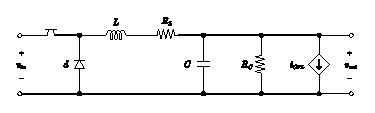
\includegraphics[scale=2.5]{figuras/buck_conversor_with_cpl_circuit.eps}
  \caption{Circuito \textit{Buck} com \acrshort{cpl}.}
  \label{fig:circuit1}
\end{figure}

% Introdução para o desenvolvimento das equações
% To-do: não esquecer de apresentar a forma completa do MMS e do MPS
% Dúvida: É para ser mais detalhista na obtenção das equações?
As equações que regem o comportamento do sistema são derivadas das leis fundamentais da eletricidade. O modelo matemático do conversor \textit{buck} se baseia no \acrshort{mms}. Apesar da natureza não linear intrínseca dos conversores, a prática usual é empregar \acrshort{mps} para obter uma representação linearizada em torno do ponto de operação. Para tal, o circuito é analisado em duas situações distintas: chave fechada e chave aberta.

% Modelagem do sistema para chave fechada
Na situação em que a chave está fechada, o circuito pode ser simplificado para um circuito série composto por uma fonte de tensão, um resistor e uma indutância, como ilustrado na \autoref{fig:circuit2}.

\begin{figure}[H]
  \centering
  % \vspace{3ex}
  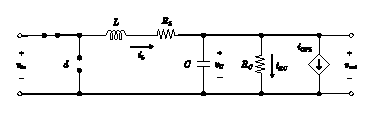
\includegraphics[scale=2.5]{figuras/buck_conversor_with_cpl_circuit_m1.eps}
  \caption{Circuito com a chave fechada.}
  \label{fig:circuit2}
\end{figure}

\noindent As equações que descrevem esse circuito são apresentadas abaixo:
% Lembrança: Faltou explica o que seria a Pcpl

\begin{equation}
  \begin{cases}
    \frac{d}{dt}i_L =  \frac{1}{L} V_{in}  - \frac{R_L}{L} i_L - \frac{1}{L} v_C \\
    \frac{d}{dt} v_C = \frac{1}{C} i_L - \frac{1}{C R_C} v_C - \frac{1}{C v_C} P_{CPL}
    \label{eq:circuito-m1}
  \end{cases}
\end{equation}
\\
\indent Na segunda situação, a chave está aberta e, consequentemente, a fonte de tensão é desconectada do circuito. Essa situação é representada na \autoref{fig:circuit3}.

\begin{figure}[H]
  \centering
  % \vspace{3ex}
  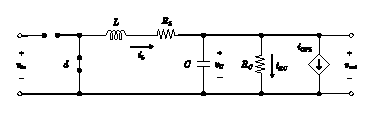
\includegraphics[scale=2.5]{figuras/buck_conversor_with_cpl_circuit_m2.eps}
  \caption{Circuito com a chave aberta.}
  \label{fig:circuit3}
\end{figure}

Neste caso, as equações que descrevem o circuito quando a chave está aberta são:

\begin{equation}
  \begin{cases}
    \frac{d}{dt}i_L  & = \frac{V_{in}}{L} d - \frac{R_L}{L} i_L - \frac{1}{L} v_C        \\
    \frac{d}{dt} v_C & = \frac{1}{C} i_L - \frac{1}{C R_C} v_C - \frac{1}{C v_C} P_{CPL}
    \label{eq:circuito-m2}
  \end{cases}
\end{equation}
\\
A partir da \autoref{eq:circuito-m1} e \autoref{eq:circuito-m2}, derivadas anteriormente, podemos estabelecer as seguintes equações diferenciais, as quais caracterizam o \acrshort{mms} e fornecem uma descrição do comportamento do circuito durante a operação contínua da chave.

\begin{equation}
  \begin{cases}
    \frac{d}{dt}i_L  & = \frac{V_{in}}{L} d - \frac{R_L}{L} i_L - \frac{1}{L} v_C        \\
    \frac{d}{dt} v_C & = \frac{1}{C} i_L - \frac{1}{C R_C} v_C - \frac{1}{C v_C} P_{CPL}
    \label{eq:nonlinear-system}
  \end{cases}
\end{equation}
\\
\indent Por meio da \autoref{eq:nonlinear-system}, onde é apresentado o sistema não linear, pode-se obter o sistema linearizado em torno dos pontos de operação. Esse sistema linear é representado por um conjunto de equações diferenciais, que descrevem as variações no tempo das grandezas $\delta i_L$ e $\delta v_C$, representando as alterações na corrente do indutor e na tensão do capacitor, respectivamente.

Considerando o sistema linearizado descrito por: \begin{equation} \dot{x} = Ax(t) + B_uu(t) + B_ww(t), \end{equation} onde  $x = \begin{bmatrix} \delta i_L & \delta v_C \end{bmatrix} ^ T$ representa o estado do sistema, $u = \delta d$ é a entrada do sistema e $w = \delta P_{CPL}$ é o sinal de pertubação. Além disto, $A \in \mathbb{R}^{n \times n}$, $B_u \text{ e } B_w \in \mathbb{R}^{n \times 1}$, são obtidos por meio das matrizes jacobianas das equações em (\ref{eq:nonlinear-system}), em torno do ponto de equilíbrio $P_{eq} = ({i_L}_0, \hspace{0.07cm} {v_C}_0, \hspace{0.07cm} {d}_0, \hspace{0.07cm} {P_{CPL}}_0)$. Portanto, o sistema linearizado obtido pode ser expresso como:

\begin{equation}
  \begin{bmatrix}
    \dot{\delta i_L} \\ \dot{\delta v_C}
  \end{bmatrix}
  =
  \begin{bmatrix}
    -\frac{R_L}{L} & -\frac{1}{L}                                                                \\
    \frac{1}{C}    & \frac{1}{C}\left(\frac{{P_{CPL}}_0}{{{{v_{C}}_0}^2}} - \frac{1}{R_C}\right)
  \end{bmatrix}
  \begin{bmatrix}
    \delta i_L \\ \delta v_C
  \end{bmatrix}
  +
  \begin{bmatrix}
    {\frac{V_{in}}{L}} & 0                     \\
    0                  & {-\frac{1}{C{v_C}_0}}
  \end{bmatrix}
  \begin{bmatrix}
    \delta d \\ \delta P_{CPL}
  \end{bmatrix}
\end{equation}

\section{Simulação}

\chapter{Controle Baseado em Eventos de Conversores CC-CC} \label{cap4}

% Essa análise fornece insights sobre a aplicação das abordagens de ETC e permite comparar suas vantagens e desvantagens.


\section{Modelo de \acrshort{etm} para Sistemas Lineares}

% ETM: Apresentação do sistema dinâmico
Nesta pesquisa, é proposto um modelo de \acrshort{etm} dinâmico para sistemas lineares, representada pela equação diferencial abaixo: \begin{equation} \dot{x}(t) = Ax(t) + Bu(t). \label{eq:linear_system_etm}\end{equation} Nesta equação, $ x(t) \in \mathbb{R}^n $ representa o estado do sistema, $ u(t) \in \mathbb{R}^m $ é a entrada de controle, e $ A \in \mathbb{R}^{n \times n} $ e $ B \in \mathbb{R}^{n \times m}$ são a matriz de estados e a matriz de entrada, respectivamente. Além disto, a origem do sistema é considerada o ponto de equilíbrio de interesse.

% ETM: Apresentação do erro de transmissão
Como discutido na seção \ref{section:etm_classification}, quando uma amostra de dados é transmitida no tempo de evento $t_k$, o estado disponível para o controlador é atualizado para $\hat{x}(t) = x(t_k)$, para todo $t$ no intervalo $[t_k, t_{k+1})$. Ao utilizar um \acrshort{zoh}, $\hat{x}(t)$ é mantido constante até o próximo tempo de evento $t_{k+1}$, resultando no erro de transmissão representado por: \begin{equation}
  e(t) = \hat{x}(t) - x(t), \quad \forall t \in [t_k, t_{k+1}).
\end{equation} Este erro ocorre durante o intervalo de tempo entre eventos, $ [t_k, t_{k+1})$.

% Adicionar um conclusão

\subsection{\acrshort{etm} Estático e Dinâmico}

% Resumo sobre o ETM estático
Como discutido anteriormente, o \acrshort{etm} estático opera considerando apenas os estados atuais do sistema $x(t)$ e o erro de transmissão $e(t)$. A sua lei de acionamento de eventos é definida como: \begin{equation} t_0 = 0, t_{k+1} = \inf \{t > t_k : \Gamma(x(t), e(t)) < 0 \}, \, \forall k \in \mathbb{N},\end{equation} onde $\Gamma(x, e)$ representa a função de evento do \acrshort{etm}. Adicionalmente, para uma classe específica de funções $\Gamma$ dada por \begin{equation}
  \Gamma(x(t), e(t)) = \sigma \alpha(\|x(t)\|) - \beta(\|e(t)\|),
\end{equation} com $\sigma \in (0,1)$, o sistema em malha fechada é assintoticamente estável.

% Função evento proposta
Com base nisso, é proposta uma função de evento onde $\alpha(\|x(t)\|) = x^T(t)\Psi x(t)$, $\beta(\|e(t)\|) = e^T(t)\Xi e(t)$ e $\sigma = 1$, ou seja: \begin{equation}
  \Gamma(x(t), e(t)) = x^T(t)\Psi x(t) - e^T(t)\Xi e(t),
  \label{eq:static_etm_gamma}
\end{equation} onde $\Psi, \, \Xi \in \mathbb{R}^{n \times n}$ e a condição suficiente para o projeto do \acrshort{etm} por co-design para o \acrshort{etc} contínuo e o controlador por realimentação de estados é declarada a seguir:

\begin{theorem}
  \label{theorem:constraints-2}
  Se existirem matrizes semidefinidas positivas $\Xi, \Psi, X \in \mathbb{R}$ e uma matriz $\tilde{K} \in \mathbb{R}^{m \times n}$ que satisfaçam a seguinte \acrshort{lmi}:
  \begin{equation}
    \begin{bmatrix}
      \mathrm{He}(AX +B\tilde{K}) & B\tilde{K}   & X             \\
      \star              & -\tilde{\Xi} & 0             \\
      \star              & \star        & -\tilde{\Psi}
    \end{bmatrix} < 0,
    \label{eq:etm_lmi_1}
  \end{equation}
  então, a origem do sistema de malha fechada é assintoticamente estável com $K = \tilde{K}X^{-1}$, $\Xi= X^{-1}\tilde{\Xi}X$, $\Psi = \tilde{\Psi}^{-1}$, $P = X^{-1}$ e a função de Lyapunov $V(x)=x^TPx$.
\end{theorem}

% ETM: Tempo de ocorrência dos eventos e a variável interna dinâmica
No \acrshort{etm} dinâmico, a lei de acionamento de eventos é definida como: \begin{equation} t_0 = 0, t_{k+1} = \inf \{t > t_k : \eta(t) + \theta \Gamma(x(t), e(t) < 0) \}, \, \forall k \in \mathbb{N} \end{equation} onde $\theta \in \mathbb{R}_{\geq 0}$ é um parâmetro de projeto, a função de evento $\Gamma(x, e)$ é a mesma definida para o \acrshort{etm} estático, em \eqref{eq:static_etm_gamma} e $\eta$ é a variável dinâmica definida por: \begin{equation}  \dot{\eta} = - \lambda \eta(t) + \Gamma(x(t), e(t)), \label{eq:dynamic-etm}\end{equation} onde $\lambda \in R_{\geq} 0 $ é o parâmetro de projeto relacionado à taxa de decaimento de $\eta(t)$.

% ETM: Condições de Co-design
\subsection{Minimização do número de eventos}


Para reduzir o número de eventos gerados, é proposto o seguinte problema de otimização convexa que visa minimizar $\lambda_{\max} (\Xi)$ e maximizar $\lambda_{\min}(\Psi)$: \begin{equation}\underset{Q, X, \tilde{\Xi}, \tilde{\Psi}, \tilde{K}}\min \quad \mathbf{tr}(\tilde{\Xi} + \tilde{\Psi} + Q). \label{eq:optimization_problem}\end{equation} Este problema é sujeito a \acrshort{lmi} apresentada em \eqref{eq:etm_lmi_1} e à seguinte \acrshort{lmi}: \begin{equation}\begin{bmatrix}
  -Q & I \\ \star & -X
\end{bmatrix} < 0. \label{eq:constraints_2}\end{equation} A solução deste problema tende a minimizar os autovalores de $Q$, $\tilde{\Xi}$ e $\tilde{\Psi}$ e a aumentar o intervalo de tempo entre os eventos. Se o problema for factível, é possível determinar as variáveis do problema e obter os parâmetros de projeto do \acrshort{etm} capazes de reduzir o número de transmissões geradas pelo \acrshort{etm}.

\section{Conversores em Malha Fechada sob o \acrshort{etm}}
\include{parte2_textuais/cap5_conclusão}

\bibliographystyle{IEEEtranN} % Ordem de citação
%\bibliographystyle{humannat} % Ordem alfabética
%\bibliographystyle{dinat}    % Ordem alfabética
%\bibliographystyle{plainnat} % Ordem alfabética
%\bibliographystyle{apa}      % Ordem alfabética

\bibliography{referencias.bib}


\appendix

\chapter{Simulação de Sistemas Dinâmicos usando Python} \label{apendice_a}


% Introdução
Nesta apêndice, é apresentado o passo a passo para simulação de sistemas dinâmicos utilizando a linguagem de programação Python e bibliotecas específicas para simulação de sistemas dinâmicos. O pacote \textit{Python Control Systems Library} é utilizado para simular os sistemas dinâmicos, enquanto o \textit{NumPy} é utilizado para a computação científica e o \textit{Matplotlib} para a visualização dos resultados.

\section{Criação de Sistemas}

Neste seção será explorado a criação de sistemas lineares e não lineares. Para isto, é utilizada a função \texttt{control.ss()} da biblioteca \textit{Python Control Systems Library}. A função \texttt{control.ss()} aceita diferentes conjuntos de parâmetros para criar sistemas dinâmicos que serão discutidos a seguir.

\subsection{Sistema Não Lineares}

Para criar um sistema não linear, utiliza-se a opção completa a seguir:

\begin{lstlisting}[language=Python]
  control.ss(updfcn, outfcn, inputs, outputs, states, dt, name, params)
\end{lstlisting}

Essa função cria um sistema de entrada/saída não linear com uma função de atualização \texttt{updfcn} e uma função de saída \texttt{outfcn}. Essa opção é utilizada para especificar um sistema não linear por meio de uma função de atualização de estado e uma função de saída. O sistema pode ser contínuo ou discreto no tempo.

A função \texttt{updfcn(t, x, u, params) $\rightarrow$ \textit{array}} é um objeto \textit{callable} que retorna a função de atualização de estado. Esta função de atualização deve retornar as derivadas dos estados por meio das equações dinâmicas do sistema não linear. Aqui, \texttt{x} é um \textit{array} unidimensional que representa os estados do sistema, \texttt{u} é um \textit{array} unidimensional que representa as entradas do sistema, \texttt{t} é uma variável de ponto flutuante que indica o tempo atual, e \texttt{params} é um dicionário contendo os valores dos parâmetros utilizados pela função. Já a função \texttt{outfcn(t, x, u, params) $\rightarrow$ \textit{array}} é uma função que fornece a saída no estado especificado. Os argumentos são os mesmos que os de \texttt{upfcn}.

\texttt{inputs} descreve as entradas do sistema. Pode ser definido com um valor inteiro que indica a quantidade de entradas do sistema, ou como uma lista de strings que nomeiam os sinais individualmente. Se for definido como um valor inteiro, os nomes dos sinais individuais serão automaticamente definidos como \texttt{u[i]}, onde \texttt{i} é a posição do sinal na lista de entradas do sistema.

\texttt{states} descreve os estados do sistema. Pode ser definido com um valor inteiro que indica a quantidade de estados do sistema, ou como uma lista de strings que nomeiam os sinais individualmente. Se for definido como um valor inteiro, os nomes dos sinais individuais serão automaticamente definidos como \texttt{x[i]}, onde \texttt{i} é a posição do sinal na lista de estados do sistema.

\texttt{outputs} descreve as saídas do sistema. Pode ser definido com um valor inteiro que indica a quantidade de saídas do sistema, ou como uma lista de strings que nomeiam os sinais individualmente. Se for definido como um valor inteiro, os nomes dos sinais individuais serão automaticamente definidos como \texttt{y[i]}, onde \texttt{i} é a posição do sinal na lista de saídas do sistema.

\texttt{name} representa o nome do sistema, o qual pode ser usado para diferenciar os sinais do sistema quando conectado a outros sistemas. Se não especificado, um nome genérico \texttt{<sys[id]>} é gerado com um identificador inteiro único.

\texttt{params} é um dicionário que armazena os valores dos parâmetros necessários para o sistema. Este dicionário é compartilhado com todas as funções de avaliação do sistema.

\subsection{Sistema Lineares}

Os sistemas dinâmicos lineares invariantes no tempo são sistemas que podem ser representados por meio do espaço de estados definidos da seguinte forma: \begin{equation}
  \begin{cases}
    \dt{x}(t) = Ax(t) + Bu(t) \\
    y = Cx(t) + Du(t)
  \end{cases},
  \label{eq:sim_space_model}
\end{equation} onde $x(t) \in \mathbb{R}^{n \times 1}$ é o vetor de estados do sistema, $u(t) \in \mathbb{R}^{m \times 1}$ é o vetor de entradas do sistema, $y(t) \in \mathbb{R}^{l \times 1}$ é o vetor de saídas do sistema, $A \in \mathbb{R}^{n \times n}$ é matriz de estados, $B \in \mathbb{R}^{n \times m}$ é a matriz de entradas, $C \in \mathbb{R}^{l \times n}$ é a matriz de saídas e $D \in \mathbb{R}^{l \times m}$ é a matriz de alimentação.

Dessa forma, para representar um sistema linear invariante no tempo, é possível utilizar a seguinte opção \texttt{control.ss(A, B, C, D[, dt])}. Nesta função, \texttt{A}, \texttt{B}, \texttt{C} e \texttt{D} são \textit{\textit{array}s} que representam as matrizes do sistema \eqref{eq:sim_space_model}, enquanto \texttt{dt} indica se o sistema é contínuo (\texttt{dt = 0}) ou discreto (\texttt{dt > 0}), sendo \texttt{dt} o tempo de amostragem. Esta opção de \texttt{ss()} também aceita os demais parâmetros descritos para a criação de sistemas não lineares na seção anterior, Além disto, é possível criar um sistema linear usando a mesma abordagem da criação de sistemas não lineares por meio das funções \texttt{updfcn} e \texttt{outfcn}, que pode ser útil em determinados casos.

\subsection{Interconexão de sistemas}

Para criar sistemas interconectados utilizando um conjunto de sistemas já criados, é possível utilizar a função \texttt{control.interconnect()}. Esta função aceita os seguinte principais parâmetros: \texttt{syslist}, \texttt{connections}, \texttt{inplist}, \texttt{outlist}, \texttt{inputs}, \texttt{outputs},  \texttt{states} e \texttt{params}.

\texttt{syslist} é a lista de sistemas que serão conectados. O parâmetro \texttt{connections} consiste em uma lista que descreve as conexões internas entre os subsistemas. Cada conexão é representada por uma lista que detalha uma entrada para um dos subsistemas. As conexões podem ser representadas de várias formas, sendo a mais básica por um par ordenado \texttt{('sys', 'sig') or ('sys', 'sig', gain)}, onde \texttt{'sig'} é um sinal de saída que será conectada a entrada \texttt{'sig'} com um ganho \texttt{gain}. Se o ganho for omitido, então ele será considerado igual a 1.

\texttt{inplist} é uma lista de conexões que determina como as entradas para o sistema global são mapeadas para as entradas dos subsistemas. 

\texttt{outlist} é uma lista de conexões que determina como as saídas dos subsistemas são mapeadas para as saídas do sistema global.

\texttt{inputs} descreve as entradas do sistema. Pode ser fornecido como um número inteiro ou como uma lista de strings que nomeiam os sinais individuais. Se fornecido como um número inteiro, os nomes dos sinais serão gerados na forma \texttt{u[i]}.

\texttt{outputs} descreve as saídas do sistema. Pode ser fornecido como um número inteiro ou como uma lista de strings que nomeiam os sinais individuais. Se fornecido como um número inteiro, os nomes dos sinais serão gerados na forma \texttt{y[i]}.

\texttt{states} descreve os estados do sistema. Pode ser fornecido como um número inteiro ou como uma lista de strings que nomeiam os sinais individuais. Se fornecido como um número inteiro, os nomes dos sinais serão gerados na forma \texttt{x[i]}.

4. \texttt{params} é um dicionário que fornece os valores dos parâmetros para os sistemas compartilhado com todas as funções do sistema.

\section{Exemplos}

\subsection{Sistema Massa-Mola}

Considere o seguinte sistema dinâmico massa-mola:

\begin{figure}[H]
  \centering
  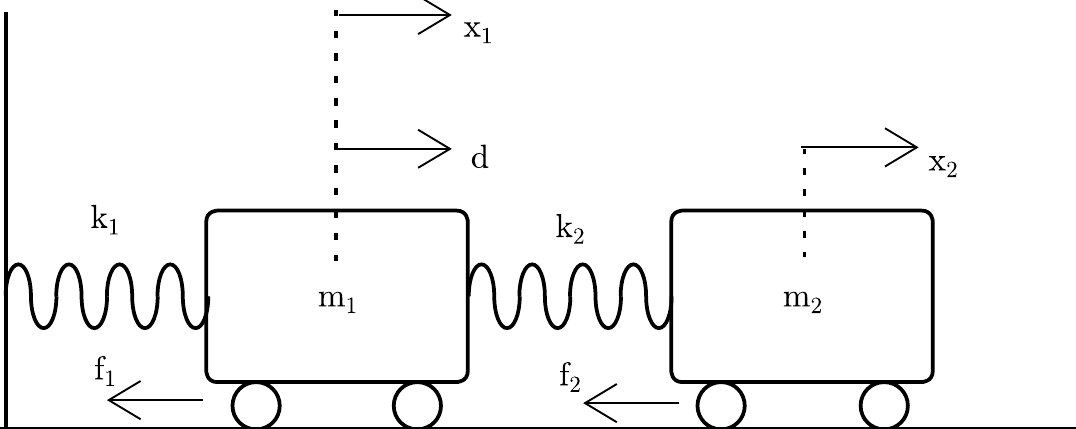
\includegraphics[width=0.8\textwidth]{figuras/sistema_massa_mola.png}
  \caption{Sistema massa-mola.}
  \label{fig:sistema_massa_mola}
\end{figure}

A sua representação no espaço de estados considerando a força $d(t)$ aplicada à massa $m_1$ como sinal de entrada e as posições $x_1(t)$ e $x_2(t)$ como saída do sistema, conforme a seguinte equação: \begin{gather}
  \begin{bmatrix}
    \dot{x_1} \\ \dot{x_2} \\ \ddot{x_1} \\ \ddot{x_2}
  \end{bmatrix}
  =
  \begin{bmatrix}
    0                                   & 0                             & 1                             & 0                             \\
    0                                   & 0                             & 0                             & 1                             \\
    \displaystyle-\frac{k_1 + k_2}{m_1} & \displaystyle\frac{k_2}{m_1}  & \displaystyle-\frac{c_0}{m_1} & 0                             \\
    \displaystyle\frac{k_2}{m_2}        & \displaystyle-\frac{k_2}{m_2} & 0                             & \displaystyle-\frac{c_0}{m_2}
  \end{bmatrix}
  \begin{bmatrix}
    x_1 \\ x_2 \\ \dot{x_1} \\ \dot{x_2}
  \end{bmatrix}
  +
  \begin{bmatrix}
    0                           \\
    0                           \\
    \displaystyle \frac{1}{m_1} \\
    0                           \\
  \end{bmatrix}
  d \\[12pt]
  y =
  \begin{bmatrix}
    1 & 0 & 0 & 0 \\
    0 & 1 & 0 & 0
  \end{bmatrix}
  \begin{bmatrix}
    x_1 \\ x_2 \\ \dot{x_1} \\ \dot{x_2}
  \end{bmatrix}
\end{gather}

Portanto, as matrizes $A$, $B$ e $C$ e $D$ são dadas por: \begin{equation}
  A = \begin{bmatrix}
    0                                   & 0                             & 1                             & 0                             \\
    0                                   & 0                             & 0                             & 1                             \\
    \displaystyle-\frac{k_1 + k_2}{m_1} & \displaystyle\frac{k_2}{m_1}  & \displaystyle-\frac{c_0}{m_1} & 0                             \\
    \displaystyle\frac{k_2}{m_2}        & \displaystyle-\frac{k_2}{m_2} & 0                             & \displaystyle-\frac{c_0}{m_2}
  \end{bmatrix}
  , \space
  B =
  \begin{bmatrix}
    0                           \\
    0                           \\
    \displaystyle \frac{1}{m_1} \\
    0                           \\
  \end{bmatrix}
  , \space
  C =
  \begin{bmatrix}
    1 & 0 & 0 & 0 \\
    0 & 1 & 0 & 0
  \end{bmatrix}
  , \space
  D = 0
\end{equation}

O \autoref{cod:sistema_massa_mola} apresenta um exemplo de como implementar este sistema dinâmico considerando os seguintes valores para parâmetros do sistema: massas $m_1 = 1$ e $m_2 = 0.5$; elasticidade das molas $k_1 = k_2 = 1$; e as forças de atrito $f_1$ e $f_2$ são determinadas por $f_i = -c_0 \cdot \dot{x_i}$, onde $i = 1, 2$. Aqui, $c_0 = 2$ representa o coeficiente de atrito viscoso. E a \autoref{fig:result_sistema_massa_mola} apresenta as figuras obtidas na simulação do sistema massa-mola.

\vspace{8pt}
\begin{lstlisting}[language=Python, caption={Código de simulação do sistema massa-mola.}, label=cod:sistema_massa_mola]
import control as ct
import numpy as np
import matplotlib.pyplot as plt


# Definição dos Parâmetros
m1 = 1.
m2 = 0.5
k1 = 1.
k2 = 1.
c0 = 2.

# Matrizes do sistema massa-mola
A = [
    [0., 0., 1., 0.],
    [0., 0., 0., 1.],
    [-((k1 + k2) / m1), (k2 / m1), - (c0 / m1), 0.],
    [(k2 / m2), - (k2 / m2), 0., - (c0 / m2)]
]

B = [[0.], [0.], [1. / m1], [0.]]

C = [[1, 0, 0, 0], [0, 1, 0, 0]]

D = 0

# Definição do sistema mass-mola
system = ct.ss(
    A, B, C, D,
    name='Sistema Massa-mola',
    inputs=('d'),
    states=('x1', 'x2', 'x1_dot', 'x2_dot'),
    outputs=('x1', 'x2', )
)

# Simulação do sistema

# Tempo de simulação: 0 a 60 segundos, com 100 pontos
timepts = np.linspace(0, 60, 100)

t, y = ct.input_output_response(
    sys=system, T=timepts,
    U=1,
    X0=[0, 0, 0, 0],
)

# Apresentação dos resultados

# Criação e apresentação dos gráficos
fig, axs = plt.subplots(1, 2, figsize=(12, 4))

# Obtenção da saída x1
x1 = y[system.find_output('x1')]

# Gráfico 1 - x1
axs[0].plot(
    t, x1,
    linestyle='-', color='#120a8f', label='$\delta i_L$',
)

axs[0].set_xlabel('Tempo(s)')
axs[0].set_ylabel('Valores de $\delta i_L\,(A)$')
axs[0].set_title('Posição $x_1$')
axs[0].legend()
axs[0].grid(True)

# Obtenção da saída x2
x2 = y[system.find_output('x2')]

# Gráfico 2 - x2
axs[1].plot(
    t, x2,
    linestyle='-', color='#8b0000', label='$\delta v_C$',
)

axs[1].set_xlabel('Tempo(s)')
axs[1].set_ylabel('Valores de $\delta v_C\,(V)$')
axs[1].set_title('Posição $x_2$')
axs[1].legend()
axs[1].grid(True)

fig.suptitle('Sistema Dinâmico Massa-mola', fontsize=16)

plt.tight_layout()
plt.show()

plt.savefig('sistema_massa_mola.eps', format='eps', bbox_inches='tight')

\end{lstlisting}

\begin{figure}[H]
  \centering
  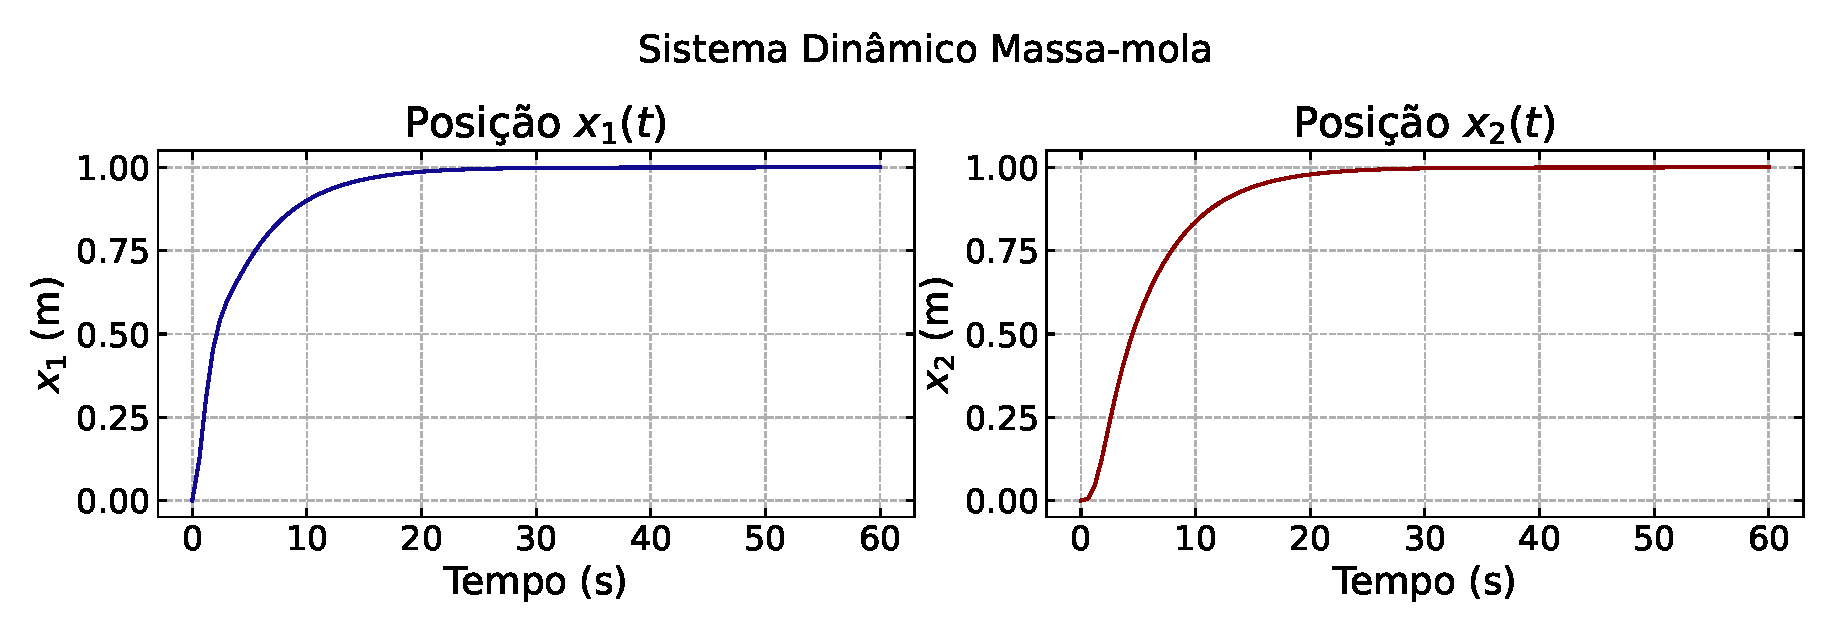
\includegraphics[width=1.\textwidth]{figuras/apendices/A/result.eps}
  \caption{Saídas do sistema massa-mola.}
  \label{fig:result_sistema_massa_mola}
\end{figure}

\subsection{Conversor \acrshort{cc}-\acrshort{cc} \textit{Buck} Não Linear e Linearizado} \label{seção_apendice_a_conversor_buck}

Neste exemplo, é apresentada a implementação e simulação de um Conversor \acrshort{cc}-\acrshort{cc} \textit{Buck} não linear, cujo circuito é ilustrado na figura a seguir:

\begin{figure}[H]
  \centering
  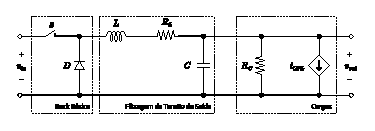
\includegraphics[width=1.\textwidth]{figuras/buck_converter_circuit.eps}
  \captionsetup{justification=centering}
  \caption{Conversor \acrshort{cc}-\acrshort{cc} \textit{Buck} básico com filtragem de tensão de saída conectado a uma \acrshort{crl} e uma \acrshort{cpl}}
  \label{eq:apendice_circuito_buck}
\end{figure}

O seu modelo dinâmico médio não linear é definido como: \begin{equation}\begin{cases} \dt{i}_L &= \displaystyle - \frac{R_L}{L} i_L(t) - \frac{1}{L} v_C(t) + \frac{v_{\mathrm{in}}}{L}d(t)  \\[8pt] \dt{v}_C &= \displaystyle \frac{1}{C} i_L(t) - \frac{1}{C R_C} v_C(t) - \frac{1}{C v_C(t)} P_{\mathrm{cpl}}(t) \label{eq:buck_nonlinear_system} \end{cases}.\end{equation} E seu modelo linearizado em torno do ponto de operação $P_{\mathrm{o}} = \left({i_L}_{\mathrm{o}}, \, {v_C}_{\mathrm{o}}, \, d_{\mathrm{o}}, \, {P_{\mathrm{cpl}}}_{\mathrm{o}} \right)$, onde \begin{equation}\begin{aligned}
    {i_L}_{\mathrm{o}} = \frac{1}{R_C} {v_C}_{\mathrm{o}} + \frac{1}{{v_C}_{\mathrm{o}}} {P_{\mathrm{cpl}}}_{\mathrm{o}} 
     \hspace{1cm}&
    d_{\mathrm{o}} = \frac{R_L}{v_{\mathrm{in}}} {i_L}_{\mathrm{o}} + \frac{{v_C}_{\mathrm{o}}}{v_{\mathrm{in}}}
    \label{eq:operation_point},
  \end{aligned}
\end{equation} é representado pelo seguinte espaço de estados: \begin{equation} \begin{bmatrix} \dt{\delta i_L} \\ \dt{\delta v_C} \end{bmatrix} = \begin{bmatrix} \displaystyle -\frac{R_L}{L} & \displaystyle -\frac{1}{L}  \\[12pt] \displaystyle \frac{1}{C} & \displaystyle \frac{1}{C}\left(\frac{{P_{\mathrm{cpl}}}_{\mathrm{o}}}{{{v_{C}}^2_{\mathrm{o}}}} - \frac{1}{R_C}\right) \end{bmatrix} \begin{bmatrix} \delta i_L(t) \\ \delta v_C(t) \end{bmatrix} + \begin{bmatrix} {\displaystyle \frac{v_{\mathrm{in}}}{L}} & 0 \\[12pt] 0 & \displaystyle {-\frac{1}{C{v_C}_{\mathrm{o}}}} \end{bmatrix}  \begin{bmatrix} \delta d(t) \\ \delta P_{\mathrm{cpl}}(t) \end{bmatrix}. \label{eq:buck_sistema_linearizado}\end{equation} Com base nessas equações, é possível simular o seu comportamento dinâmico computacionalmente, como será apresentados nos próximos passos.

Primeiramente, serão definidos os parâmetros do conversor \textit{Buck} necessários para a sua implementação. Para isto, é criada uma variável \texttt{params} que é um dicionário que conterá os parâmetros do conversor. No conversor \textit{Buck}, os parâmetros são a tensão de entrada (\texttt{Vin}), as resistências (\texttt{rL} e \texttt{rC}), a indutância (\texttt{L}), a capacitância (\texttt{C}), a potência da CPL e a tensão desejada do capacitor (\texttt{Pcpl} e \texttt{vC}). Em seguida, são calculadas a corrente do indutor (\texttt{iL}) e o ciclo de trabalho (\texttt{d}) no ponto de operação, de acordo com as relações expressas em \eqref{eq:operation_point}. Com esses valores do ponto de operação, as entradas \texttt{U\_OP} e os estados \texttt{X\_OP} são definidos. Além disso, a entrada do sistema (\texttt{U}) é definida como os valores no ponto de operação, enquanto os estados iniciais (\texttt{X0}) são definidos como 95\% dos valores no ponto de operação. Por fim, são calculadas as variações nas entradas (\(\delta U\)) e nos estados iniciais ($\delta X0$) em relação ao ponto de operação. A definição completa dos parâmetros do conversor \textit{Buck} está implementada no código a seguir:

\vspace{8pt}
\begin{lstlisting}[language=Python, caption={Parâmetros do conversor \textit{Buck}.}, label=cod:buck_params]
  # Parâmetros do Circuito
  params = {'Vin': 48, 'rL': 0.1, 'rC': 35,
            'L': 40e-3, 'C': 10e-6, 'op': {'Pcpl': 15, 'vC': 24}}

  # Cálculo da Corrente e Duty Cycle de Operação
  op = params['op']
  IL_OP = (op['vC'] / params['rC']) + op['Pcpl'] / op['vC']
  D_OP = (params['rL'] * IL_OP) / params['Vin'] + op['vC'] / params['Vin']

  params['op']['iL'] = IL_OP
  params['op']['d'] = D_OP

  # Ponto de operação de cada entrada e estado do sistema
  U_OP = np.\textit{array}([params['op']['d'], params['op']['Pcpl']])
  X_OP = np.\textit{array}([params['op']['iL'], params['op']['vC']])

  # Entradas do Sistema
  D = params['op']['d']
  P_CPL = params['op']['Pcpl']
  U = np.\textit{array}([D, P_CPL])

  # Estados Iniciais do Sistema
  IL_INIT = 0.95 * params['op']['iL']
  VC_INIT = 0.95 * params['op']['vC']
  X0 = np.\textit{array}([IL_INIT, VC_INIT])

  δU = U - U_OP
  δX0 = X0 - X_OP
\end{lstlisting}

% Implementação do \textit{Buck} não linear
No código \ref{cod:buck_nonlinear}, é apresentada a implementação da função de atualização dos estados e da função de saída do conversor \textit{Buck}, além da criação de um objeto que representa o sistema dinâmico. A função \texttt{update\_buck\_nonlinear} estabelece o comportamento dinâmico do conversor \textit{buck} não linear conforme expresso em \eqref{eq:apendice_circuito_buck}. Esta função recebe como entrada o tempo \texttt{t}, os estados do sistema \texttt{x}, as entradas do sistema \texttt{u} e os parâmetros do sistema \texttt{params}. A partir dessas informações, são calculadas as derivadas dos estados do sistema, que representam as mudanças da corrente do indutor \texttt{diL} e da tensão do capacitor \texttt{dvC}. Além disso, a função \texttt{output\_buck\_nonlinear} é responsável por definir quais variáveis do sistema serão consideradas como saídas, recebendo os mesmos parâmetros da função de atualização dos estados. Dessa forma, ela retorna um vetor com as variáveis de interesse, neste caso, a corrente do indutor \texttt{iL} e a tensão do capacitor \texttt{vC}. Por fim, a variável \texttt{nonlinear\_system} define um sistema de tempo contínuo utilizando a função \texttt{ct.ss}.

\vspace{8pt}
\begin{lstlisting}[language=Python, caption={Implementação do conversor \textit{Buck} não linear.}, label=cod:buck_nonlinear]
def update_buck_nonlinear(t, x, u, params):
  # Parâmetros do sistema
  V_IN = params.get('Vin')  # Tensão de Entrada
  RL = params.get('rL')     # Resistência (indutor)
  RC = params.get('rC')     # Resistência (capacitor)
  L = params.get('L')       # Indutância
  C = params.get('C')       # Capacitância

  # Entradas do sistema: Duty Cycle e Potência da CPL
  D, P_CPL = u

  # Estados do sistema: corrente do indutor e tensão do capacitor
  IL, VC = x

  # Atualização da corrente do indutor
  diL = (V_IN / L) * D - (RL / L) * IL - VC / L  

  # Atualização da tensão do capacitor   
  dvC = IL / C - VC / (C * RC) - P_CPL / (C * VC)

  dx = np.\textit{array}([diL, dvC])
  return dx

# Definição da saída do sistema
def output_buck_nonlinear(t, x, u, params):
  return x[0:2]

# Definição do conversor cc-cc \textit{buck} nao-linear
buck_nonlinear = ct.ss(
  update_buck_nonlinear, 
  output_buck_nonlinear,
  name='buck_nonlinear',
  inputs=('d', 'P_cpl'),
  outputs=('iL', 'vC'),
  states=('iL', 'vC')
)
\end{lstlisting}

O código \ref{cod:buck_linear} implementa a linearização do conversor \textit{Buck} em torno do ponto de operação $P_o$. A variável \texttt{OP} armazena os valores de $P_o$ contida no dicionário \texttt{params} e, portanto, representa o ponto de operação do conversor. Em seguida, são construídas as matrizes de estado \texttt{A}, de entrada \texttt{B}, de saída \texttt{C} e de alimentação \texttt{D} do sistema, de acordo com a linearização do conversor \textit{Buck} definida. Por último, a variável \texttt{buck\_linearized} é criada por meio da transformação do sistema linear, construído com base nas matrizes do sistema, para sua forma de representação entrada-saída. Isso é feito para aumentar a flexibilidade da simulação, permitindo a definição de tags para as entradas, saídas e estados, o que facilita a interconexão entre os sistemas.

\vspace{8pt}
\begin{lstlisting}[language=Python, caption={Implementação do conversor \textit{Buck} linearizado.}, label=cod:buck_linear]
  # Obtenção dos valores no ponto de operação (OP)
  OP = params['op']

  # Elementos da matriz de estados
  A11 = - (params['rL'] / params['L'])
  A12 = - (1. / params['L'])
  A21 = 1. / params['C']
  A22 = (1. / params['C']) * (OP['Pcpl'] /
        (OP['vC'] * OP['vC']) - 1. / params['rC'])

  # Elementos da matriz de entrada
  B11 = params['Vin'] / params['L']
  B12 = 0.
  B21 = 0.
  B22 = - 1.0 / (params['C'] * OP['vC'])

  # Matriz de estados: iL e vC
  A = [[A11, A12], [A21, A22]]

  # Matriz de entradas: d e P_cpl
  B = [[B11, B12], [B21, B22]]

  # Matriz de saída: iL e vC
  C = [[1., 0], [0., 1]]

  # Matriz de alimentação: nula
  D = [[0., 0.], [0., 0.]]

  buck_linearized = ct.ss(
    A, B, C, D,
    name='buck_linearized',
    inputs=('δd', 'δPcpl'),
    outputs=('δiL', 'δvC'),
    states=('δiL', 'δvC')
  )
\end{lstlisting}

\subsection{Conversor \textit{Buck} \acrshort{cc}-\acrshort{cc} em Malha Fechada sob \acrshort{etc}}

Neste exemplo será detalhado a implementação do conversor \textit{Buck} linearizado, definido no exemplo anterior, em malha fechada sob o \acrshort{etc}. Para isto, é realizada a interconexão entre a planta (conversor \textit{Buck}), o \acrshort{etm}, o \acrshort{zoh} e o controlador por realimentação de estados.

A partir dos parâmetros de projetos obtidos por meio da abordagem proposta neste trabalho, é implementado o \acrshort{etm} estático, cujo código está apresentado em \ref{cod:static_etm}. Este possui quatro entradas, das quais as duas primeiras são os últimos estados enviados $\hat{x}$ provenientes do ZOH e os estados atuais $x$ obtidos da planta. Suas saídas consistem em $\Gamma$, uma variável \textit{booleana} que, quando verdadeira, aciona um evento, e os estados atuais da planta. Essas saídas são determinadas pela função \texttt{etm\_output}, a qual recebe como parâmetros o tempo atual da simulação, o estado atual do \acrshort{etm}, a entrada do \acrshort{etm} e os parâmetros do sistema, respectivamente.

Internamente, a função verifica o início da segunda simulação. Isso se deve ao fato de que a simulação é realizada duas vezes: a segunda vez com um passo de simulação maior e menos preciso. Esta distinção é crucial, pois o tempo de acionamento de eventos é registrado apenas na primeira simulação, que utiliza um passo de tempo menor e mais preciso. Além disso, o cálculo de $\Gamma$ é realizado, sendo este um valor real. Caso seja negativo, um novo evento deve ser acionado. Se isso ocorrer, os estados atuais serão definidos como a saída do \acrshort{etm}; caso contrário, serão os últimos estados enviados.

\vspace{8pt}
\begin{lstlisting}[language=Python, caption={Implementação do \acrshort{etm} estático.}, label=cod:static_etm]
  zero = 0
  event_times = [0.]

  def get_gama(current_states, last_states_sent):
    error = last_states_sent - current_states
    return current_states.T @ Ψ @ current_states - error.T @ Ξ @ error


  def etm_output(t, x, u, params):
    global zero, event_times

    if t != etm_output.previous_time:
      etm_output.previous_time = t
      if etm_output.first_simulation and t == 0.:
        etm_output.first_simulation = False

    last_states_sent = u[0:2]
    current_states = u[2:4]

    Γ = get_gama(current_states, last_states_sent)
    trigger = Γ < 0

    if etm_output.first_simulation and trigger:
      event_times.append(t)

    state_to_sent = (current_states if trigger or t == 0. else last_states_sent)
    return [state_to_sent[0], state_to_sent[1]]

  etm_output.previous_time = 0
  etm_output.first_simulation = True

  ETM = ct.ss(
    None, etm_output,
    name='etm',
    inputs=('x1_hat', 'x2_hat', 'x1', 'x2'),
    outputs=('x1', 'x2'),
  )
\end{lstlisting}

No caso do \acrshort{etm} dinâmico, uma nova função, \texttt{etm\_update}, é criada. Esta função é responsável pela atualização da variável dinâmica $\eta$ do \acrshort{etm} dinâmico. Na função de saída, a lei de acionamento é modificada para incorporar a versão dinâmica do \acrshort{etm}. Além disso, uma nova saída do \acrshort{etm} é adicionada, representando a variável dinâmica do próprio \acrshort{etm}. Por fim, tanto a função de atualização quanto a saída do \acrshort{etm} dinâmico dependem dos parâmetros $\theta$ e $\epsilon$, que são previamente definidos.

\vspace{8pt}
\begin{lstlisting}[language=Python, caption={Implementação do \acrshort{etm} dinâmico.}, label=cod:dynamic_etm]
  θ = 1.
  λ = .1
  
  def etm_update(t, n, u, params):
    Γ = get_gama(current_states=u[2:4], last_states_sent=u[0:2])
    dn = -λ * n + Γ
    return [dn]


  def etm_output(t, n, u, params):
    global zero, event_times

    if t != etm_output.previous_time:
      etm_output.previous_time = t
      if etm_output.first_simulation and t == 0.:
        etm_output.first_simulation = False

    last_states_sent = u[0:2]
    current_states = u[2:4]

    Γ = get_gama(current_states, last_states_sent)
    trigger = (n + θ * Γ) < 0

    if etm_output.first_simulation and trigger:
      event_times.append(t)

    state_to_sent = (current_states if trigger or t == 0. else last_states_sent)
    return [state_to_sent[0], state_to_sent[1], n[0]]


  etm_output.previous_time = 0
  etm_output.first_simulation = True

  ETM = ct.ss(
    etm_update, etm_output,
    name='etm',
    states=('n'),
    inputs=('x1_hat', 'x2_hat', 'x1', 'x2'),
    outputs=('x1', 'x2', 'n'),
  )
  \end{lstlisting}

O código \ref{cod:zoh} é a implementação do \acrshort{zoh}. Inicialmente, é definida uma função chamada \texttt{zoh\_output}, que implementa a saída do \acrshort{zoh} para o sistema de controle contínuo. O método de saída \acrshort{zoh} retém o valor de entrada atual até o próximo instante. A função armazena o estado anterior \texttt{previous} e o tempo anterior \texttt{previous\_time}. Em cada chamada, se o tempo atual \texttt{t} for diferente do tempo anteriormente armazenado, o estado anterior é atualizado e o tempo anterior é atualizado para \texttt{t}. A função retorna os estados previamente armazenados \texttt{last\_states\_sent} que é inicializada com os valores iniciais dos estados da planta.

\vspace{8pt}
\begin{lstlisting}[language=Python, caption={Implementação do \acrshort{zoh}}, label=cod:zoh]
  def zoh_output(t, x, u, params):
    if t != zoh_output.previous_time:
      zoh_output.last_states_sent = zoh_output.previous
      zoh_output.previous_time = t
    zoh_output.previous = u
    return zoh_output.last_states_sent

  zoh_output.previous_time = 0
  zoh_output.second_simulation = False
  zoh_output.previous = []
  zoh_output.last_states_sent = δX0.tolist()

  ZOH = ct.ss(
    None, zoh_output,
    name='zoh',
    inputs=('x1', 'x2'),
    outputs=('x1_hat', 'x2_hat'),
  )
\end{lstlisting}

No código \ref{cod:controller}, é definida a função de saída do controlador, \texttt{control\_output}, responsável por implementar a operação de controle para a planta. Dentro dessa função, ocorre o cálculo do ciclo de trabalho, que consiste no produto escalar entre a matriz de ganho $K$ e os estados $\hat{x}$. Assim, a matriz de ganho representada pela variável \texttt{K} é aplicada aos estados representados por \texttt{u}, resultando no cálculo do ciclo de trabalho desejado. Este último é então retornado como saída do controlador. A seguir, é definido o sistema de controle \texttt{CONTROL}. Este sistema é estático (determinado por \texttt{None}) e utiliza a função \texttt{control\_output} como função de saída. O sistema conta com duas entradas, que correspondem aos estados provenientes do \acrshort{zoh}, e uma saída, que representa o ciclo de trabalho, entrada da planta.

\vspace{8pt}
\begin{lstlisting}[language=Python, caption={Implementação do controlador.}, label=cod:controller]
  def control_output(t, x, u, params):
    duty_cycle = K @ u
    return [duty_cycle]


  CONTROL = ct.ss(
      None, control_output,
      name='control',
      inputs=('x1_hat', 'x2_hat'),
      outputs=('u'),
  )
\end{lstlisting}

O código \ref{cod:closed_loop} cria um sistema de controle em malha fechada para o conversor \textit{Buck} sob o \acrshort{etc}. É utilizada a função \texttt{interconnect} para conectar os quatro subsistemas: o sistema linearizado do conversor \textit{Buck}, o \acrshort{etm}, o \acrshort{zoh}, e o controlador. As conexões entre esses componentes são especificadas para formar um loop de realimentação, conforme apresentado na subseção \ref{subsection:etc}. O sistema resultante é então nomeado como \texttt{closed\_loop\_buck\_system}, e suas entradas e saídas são definidas. Em seguida, define-se o tempo de simulação e o sinal de entrada, que neste caso é um sinal constante chamado \texttt{\ensuremath{\delta}Pcpl}, mas também pode ser um vetor contendo valores variados. Por fim, a função \texttt{input\_output\_response} é utilizada para simular a resposta do sistema fechado ao longo do tempo, armazenando as respostas do sistema em \texttt{t} (tempo) e \texttt{y} (saídas do sistema).

\vspace{8pt}
\begin{lstlisting}[language=Python, caption={Sistema em loop fechado sob o ETC.}, label=cod:closed_loop]
  CLOSED_LOOP_BUCK_SYSTEM = ct.interconnect(
      (buck_linearized, ETM, ZOH, CONTROL),
      connections=(
          # Conexão entre a saída do controlador e a planta
          ('buck_linearized.δd', 'control.u'),

          # Conexão entre as saídas do ZOH e da planta ao ETM
          ('etm.x1_hat', 'zoh.x1_hat'),
          ('etm.x2_hat', 'zoh.x2_hat'),
          ('etm.x1', 'buck_linearized.δiL'),
          ('etm.x2', 'buck_linearized.δvC'),

          # Conexão da saída do ETM no ZOH
          ('zoh.x1', 'etm.x1'),
          ('zoh.x2', 'etm.x2'),

          # Conexão da saída do ZOH no controlador
          ('control.x1_hat', 'zoh.x1_hat'),
          ('control.x2_hat', 'zoh.x2_hat'),
      ),
      name='closed_loop_buck_system',
      inplist=('buck_linearized.δPcpl'),
      outlist=('buck_linearized.δiL',
              'buck_linearized.δvC',
              'etm.Γ',
              'buck_linearized.δd',
              ),
      output=('δiL', 'δvC', 'Γ', 'u')
  )

  print(CLOSED_LOOP_BUCK_SYSTEM)
  print('')

  step = 1e-6
  timepts = np.arange(0, 1. + step, step)

  # Simulação para a pertubação constante
  δPcpl = 0.

  t, y = ct.input_output_response(
      sys=CLOSED_LOOP_BUCK_SYSTEM, T=timepts,
      U=δPcpl,
      X0=δX0,
      solve_ivp_method='RK45',
      solve_ivp_kwargs={'max_step': step}
  )
\end{lstlisting}
\chapter{Aquisição BDGD}\label{apendiceB}




\end{document}
